\chapter{Search for Charged Higgs Bosons}\label{chap:hpana}
	This chapter details a search for a charged Higgs boson decaying to a hadronically decaying tau lepton and a neutrino; the phenomenology is discussed in Section \ref{sec:Hpm}. This search contains two subchannels, \taujets and \taulep based on the decay of the  associated top quark in the collision event. The \taujets subchannel ($t\to Wb, \, W \to q\bar{q}$)  has a higher branching fraction, leading to higher sensitivity at larger \mHpm values. The \taulep subchannel ($t\to Wb, \, W \to \ell \nu$)  has a much lower branching fraction, but takes advantage of single-lepton triggers which enhance background suppression of QCD $\mathrm{jet} \, \to \, \tau$ fakes. This leads to an increased sensitivity at lower \mHpm values. The extra neutrino in the \taulep decay mode creates extra difficulties in separating signal from background in this subchannel by adding a significant contribution to the \Etm calculation for the event. 

	The search described by this dissertation uses a profile likelihood ratio as the test statistic in a simultaneous fit in two control regions and three signal regions. The discriminating variable is chosen to be the output score distribution of a multivariate analysis technique (MVA). In the previous publication described in Section \ref{ssec:Prev Hpm} several boosted decision trees (BDT) were used, binned in \mHpm; this analysis uses a parameterized neural network (PNN) to classify events as signal-like or background-like.

	This chapter discusses in detail the entire analysis, including the signal signatures, event selections, analyzed datasets, modeling of backgrounds, training and evaluation of classifiers, studies of systematic uncertainties, and results.

	\section{Signature and Event Selection}\label{sec:signal}
		As shown in Figure \ref{fig:hpm-diagrams}, the production of the \Hpm is dependent on the mass \mHpm. Table \ref{tab:hplus-production} shows the production mechanisms for \mHpm values with respect to the top quark mass $m_t$ as well as the main decay mode (and theoretical constraints), as well as the main source of background. Three mass ranges are defined, low mass $80 \leq \mHpm \leq 130 $ GeV, intermediate mass $140 \leq \mHpm \leq 190$, and high mass $200 \leq \mHpm \leq 3000$ GeV.  The two subchannels have similar signal signatures with a hard scatter source of \Etm, one \tauhad, and at least 1 \bjet from the associated top decay. In the \taulep subchannel there is an extra requirement of a lepton (e or $\mu$). Due to the variable amount of energy available to the final state products based on \mHpm the event topology changes as a function of \mHpm. As described in Section \ref{ssec:mva}, classifiers are trained and evaluated in \mHpm bins to account for the varying event topology.

		\begin{table}[!thp]
			\centering
			\resizebox{\textwidth}{!}{
			\begin{tabular}{| c | c | c | c |}
			\hline
			\textbf{\Hpm Mass} & \textbf{Production Mechanism} & \textbf{Decay}  & \textbf{Main Background}\\
			\hline \hline
			\multicolumn{1}{|c|}{\multirow{2}{*}{$\mHpm < m_{t}$}} 		& \begin{tabular}[c]{@{}c@{}} double-resonant $t \to H^\pm b$ (LO) \\ 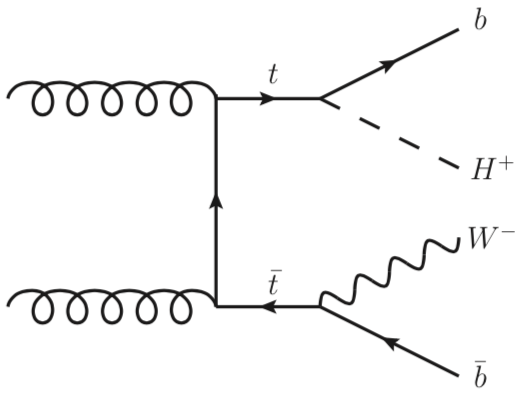
\includegraphics[width=.19\textwidth]{chapters/chapter6_HPlus/images/double_resonant_production_low_mass.png} \end{tabular} 											& \begin{tabular}[c]{@{}c@{}} \HpmLong \\ (low $\tanb \implies$ $\Hpm \to cs$ or $\Hpm \to cb$ ) \end{tabular} 																	& \ttbar, single-top \\ \hline

			\multicolumn{1}{|c|}{\multirow{3}{*}{$\mHpm \simeq m_{t}$}} & \begin{tabular}[c]{@{}c@{}} non-resonant $t \to \Hpm b$ (LO) \\ 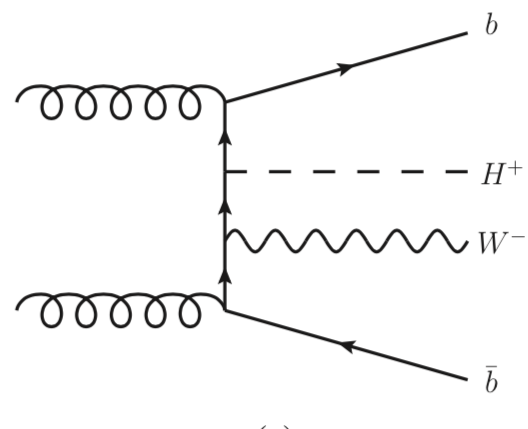
\includegraphics[width=.19\textwidth]{chapters/chapter6_HPlus/images/non_resonant_production_intermediate_mass.png} \\ interferences taken into account \end{tabular} 	& $\Hpm \to \tau \nu$  																																									& \ttbar, single-top \\ \hline

			\multicolumn{1}{|c|}{\multirow{3}{*}{$\mHpm > m_{t}$}}		& \begin{tabular}[c]{@{}c@{}} single-resonant $gg \to tbH^\pm$ (NLO) \\ 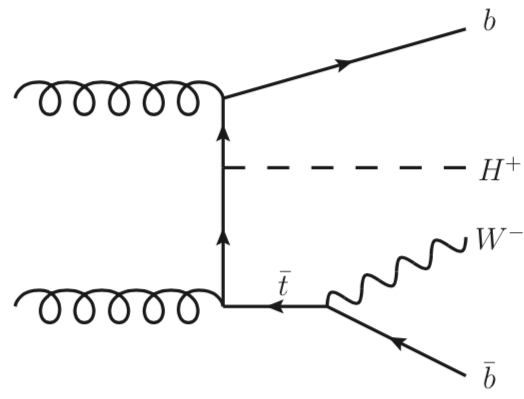
\includegraphics[width=.19\textwidth]{chapters/chapter6_HPlus/images/single_resonant_production_large_mass.png} \end{tabular} 										& \begin{tabular}[c]{@{}c@{}} $\Hpm \to tb$ \\ ($cos(\beta-\alpha) \simeq 0$ and large $tan(\beta) \implies \Hpm \to \tau \nu$ \\ $BR(\HpmLong) \simeq 10-15\%$ ) \end{tabular} & multi-jet \\ \hline

			\end{tabular}}
			\caption{\Hpm production mechanisms based on \mHpm, dominant \Hpm decay mode, and the main background associated with the diagram.}
			\label{tab:hplus-production}
		\end{table}

		\subsection{Object Definitions}\label{ssec:object-def}
		Table \ref{tab:object-defs} shows the identification requirements on all objects used in the analysis. In both subchannels \tauhad candidates are required to fit the medium working point described in Section \ref{ssec:reco-tau} that corresponds to a 75\% efficiency for 1-prong and 60\% efficiency for 3-prong \tauhad identification, an $\abs{\eta}$ cut of $< 2.3$ that also excludes the gap and crack region of the ATLAS calorimeters at $1.37 < \abs{\eta} < 1.52$, an overlap removal with electrons is also performed. For the \taujets subchannel, the \tauhad \pt is required to be greater than 40 GeV and greater than 30 GeV for the \taulep subchannel. Although muons and electrons are not part of the \taujets signal final state, a loose identification and isolation requirement is used to veto events; while the \taulep subchannel requires there to be either an electron or a muon that passes the tight identification and isolation requirements as well as a \pt above 30 GeV. The jets in candidate events are required to have greater than 25 GeV in \pt and are made with the anti-$k_t$ algorithm with R=0.4. Jets tagged as \bjets are done so at a 70\% efficient working point using the DL1r tagger described in Section \ref{ssec:flavor-tagging}.

		\begin{table}[!thp]
			\centering
			\resizebox{\textwidth}{!}{
			\begin{tabular}{| c | l | l |}
			\hline
			Object & \textbf{\taujets} & \textbf{\taulep} \\
			\hline \hline
			\multicolumn{1}{|c|}{\multirow{3}{*}{\tauhad}} & \begin{tabular}[c]{@{}c@{}}Leading reconstructed $\tau$ (regardless of its ID), \\ mediumID$^{*}$, $\pt > 40$ GeV, $\abs{\eta}^{***} < 2.3$, $e$ OLR \end{tabular} & \begin{tabular}[c]{@{}c@{}} Leading reconstructed $\tau$ (regardless of its ID), \\ mediumID$^{*}$, $\pt > 30$ GeV, $\abs{\eta}^{***} < 2.3$, $e$ OLR \end{tabular} \\[4ex] \hline
			\multicolumn{1}{|c|}{\multirow{3}{*}{$e$}} & \begin{tabular}[c]{@{}c@{}} LoseLLH, $\pt > 20$ GeV, $\abs{\eta}^{***} < 2.47$, \\ Loose isolation, IP cuts \end{tabular} &  \begin{tabular}[c]{@{}c@{}} TightLLH, $\pt > 30$ GeV, $\abs{\eta}^{***} < 2.47$, \\ Tight isolation, IP cuts \end{tabular} \\[4ex] \hline
			\multicolumn{1}{|c|}{\multirow{3}{*}{$\mu$}} & \begin{tabular}[c]{@{}c@{}} LooseID, $\pt > 20$ GeV, $\abs{\eta} < 2.5$, \\Loose isolation, IP cuts \end{tabular} & \begin{tabular}[c]{@{}c@{}} TightID, $\pt > 30$ GeV, $\abs{\eta} < 2.5$,\\ Tight isolation, IP cuts \end{tabular} \\[4ex] \hline 
			\multicolumn{1}{|c|}{\multirow{3}{*}{jet}} & \begin{tabular}[c]{@{}c@{}} AntiKt4EMPFlow, $\pt > 25$, GeV $\abs{\eta} < 2.5$,\\ JVT$^{**}$  $> 0.59$, Btag=70\%, DL1r \end{tabular} & \begin{tabular}[c]{@{}c@{}} AntiKt4EMPFlow, $\pt > 25$ GeV, $\abs{\eta} <2.5$, \\ JVT$^{**}$  $ > 0.59$ , Btag=70\%, DL1r \end{tabular} \\[4ex] \hline
			\end{tabular}}
			\caption{Definitions of physics objects used in this analysis.}
			\label{tab:object-defs}
		\end{table}

		% \begin{columns}
		% \column{.3\textwidth}
		% \begin{itemize}
		%   \footnotesize
		%   \item $\tau$ mediumID$^{*}$
		%   \begin{itemize}
		%     \tiny
		%     \item 1-prong: 75\% ID eff 
		%     \item 3-prong: 60\% ID eff
		%   \end{itemize}
		% \end{itemize}
		% \column{.3\textwidth}
		% \begin{itemize}
		%   \footnotesize
		%   \item JVT$^{**}$
		%     \begin{itemize}
		%       \tiny
		%       \item $\pt < 60$ GeV
		%       \item $\abs{\eta}<2.4$
		%   \end{itemize}
		% \end{itemize}
		% \column{.3\textwidth}
		% \begin{itemize}
		%   \footnotesize
		%   \item $\abs{\eta}^{***}$
		%     \begin{itemize}
		%       \tiny
		%       \item $1.37 < \abs{eta} < 1.52 $ excluded
		%   \end{itemize}
		% \end{itemize}
		% \end{columns}

		\subsection{Event Selections}\label{ssec:event-selection}
			Each subchannel signal region has stricter requirements than those described in Section \ref{tab:object-defs}. Table \ref{tab:signal-regions} details these selections. The channels differ in the triggers used; the \taujets subchannel relies on \Etm triggers while the \taulep subchannel relies on single lepton triggers. Due to the difficulty of separating signal from background the \taujets subchannel has a higher \pt cut on the \tauhad of 40 GeV as opposed to the \taulep value of 30 GeV. In addition, a higher value of \Etm of 150 GeV is required for the \taujets subchannel. A value of 50 GeV is also required of the transverse mass $m_{T}$ defined as 
			\begin{equation}\label{eqn:transverse-mass}
			m_{T} = \sqrt{ 2 \pt^{\tau} \Etm (1 - cos \Delta \phi_{\tau,\Etm}) }
			\end{equation}
			The \taulep has no such requirement, but does require the \tauhad and lepton to have opposite electromagnetic charge. A set of orthogonal control regions are defined for each subchannel to verify proper background modelling and are described in Section \ref{sec:bkg-modeling}. The acceptance of signal in the signal regions defined in \ref{tab:signal-regions} is shown in Figure \ref{fig:signal-acceptance}.


			\begin{table}[!thp]
				\centering
				\resizebox{.75\textwidth}{!}{
				\begin{tabular}{| c | c |}
				\hline
				\textbf{$\tau + jets$ SR } & \textbf{$\tau + \ell$ SR} \\
				\hline \hline
				$\Etm$ Trigger (mostly HLT\_xe110) & Single lepton trigger (e or $\mu$) \\[1.2ex] \hline
				1 \tauhad ; $\pt^{\tau} > 40$ GeV & 1 \tauhad ; $\pt^{\tau} > 30$ GeV\\[1.2ex] \hline
				% $\pt^{\tau} > 40$ GeV & $\pt^{\tau} > 30$ GeV \\ \hline
				0 $\ell$ (e or $\mu$) ; $\pt^{\ell} > 20$ GeV  & 1 $\ell$ (e or $\mu$) ; $\pt^{\ell} > 30$ GeV \\[1.2ex] \hline
				% $\pt^{\ell} > 20$ GeV & $\pt^{\ell} > 30$ GeV \\ \hline
				$\geq$ 3 jets ; $\pt^{j} > 25$ GeV  & $\geq$ 1 jet ; $\pt^{j} > 25$ GeV \\[1.2ex] \hline
				% $\pt^{j} > 25$ GeV & $\pt^{j} > 25$ GeV \\ \hline
				$\geq$ 1 \bjets ; $\pt^{\bjet} > 25$ GeV & $\geq$ 1 \bjets ; $\pt^{\bjet} > 25$ GeV \\[1.2ex] \hline
				% $\pt^{\bjet} > 25$ GeV & $\pt^{\bjet} > 25$ GeV \\ \hline
				\Etm$ > 150$ GeV & \Etm$ > 50$ GeV \\[1.2ex] \hline
				$m_{T}(\tau,\Etm) > 50$ GeV & Opposite sign $\tau$ and $\ell$ \\[1.2ex] 
				\hline
				\end{tabular}}
				\caption{\taujets and \taulep signal region definitions.}
				\label{tab:signal-regions}
			\end{table}

			\begin{figure}[!ht]
				\centering
				\subfloat[\label{fig:signal-acceptance_a}]{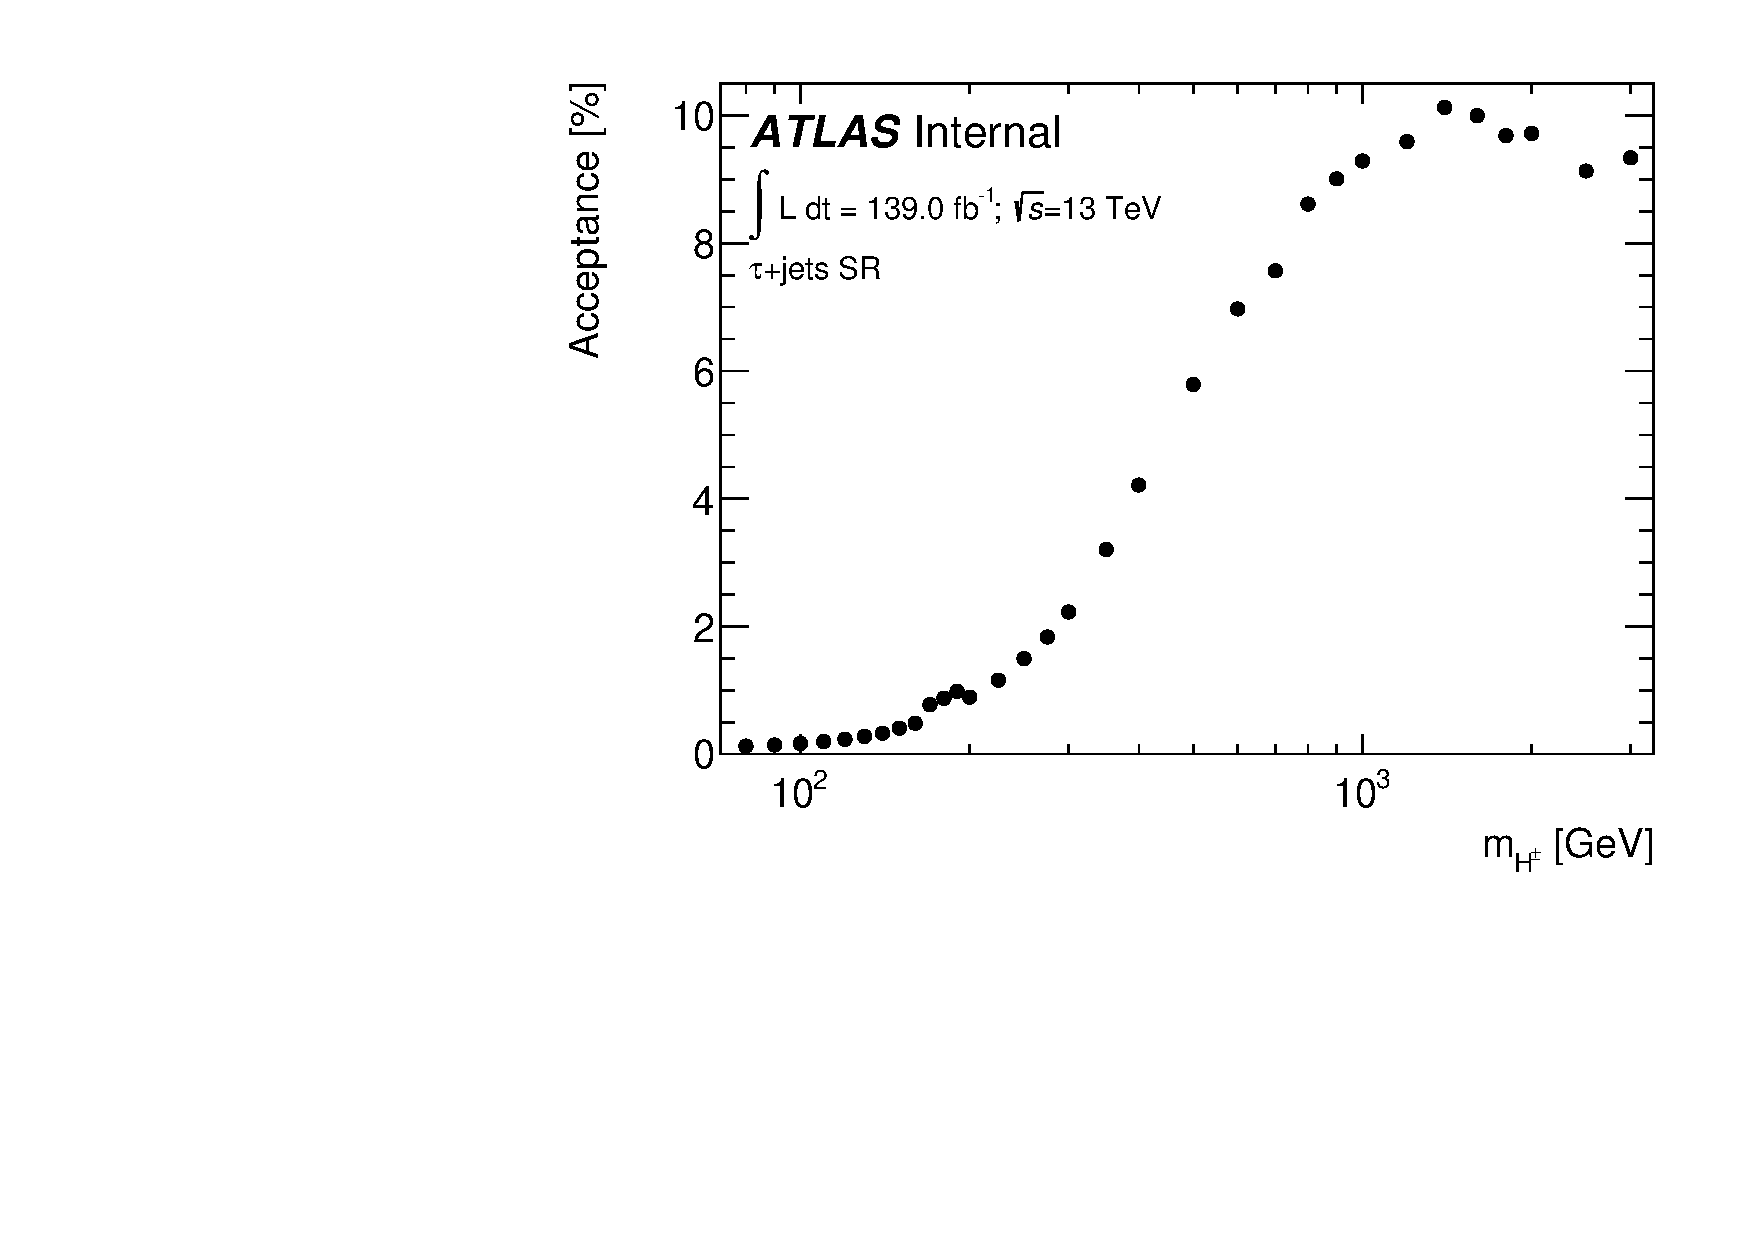
\includegraphics[width=0.5\textwidth]{chapters/chapter6_HPlus/images/Signal_Acceptance_Efficiency_SR_TAUJET.pdf}}
				\subfloat[\label{fig:signal-acceptance_b}]{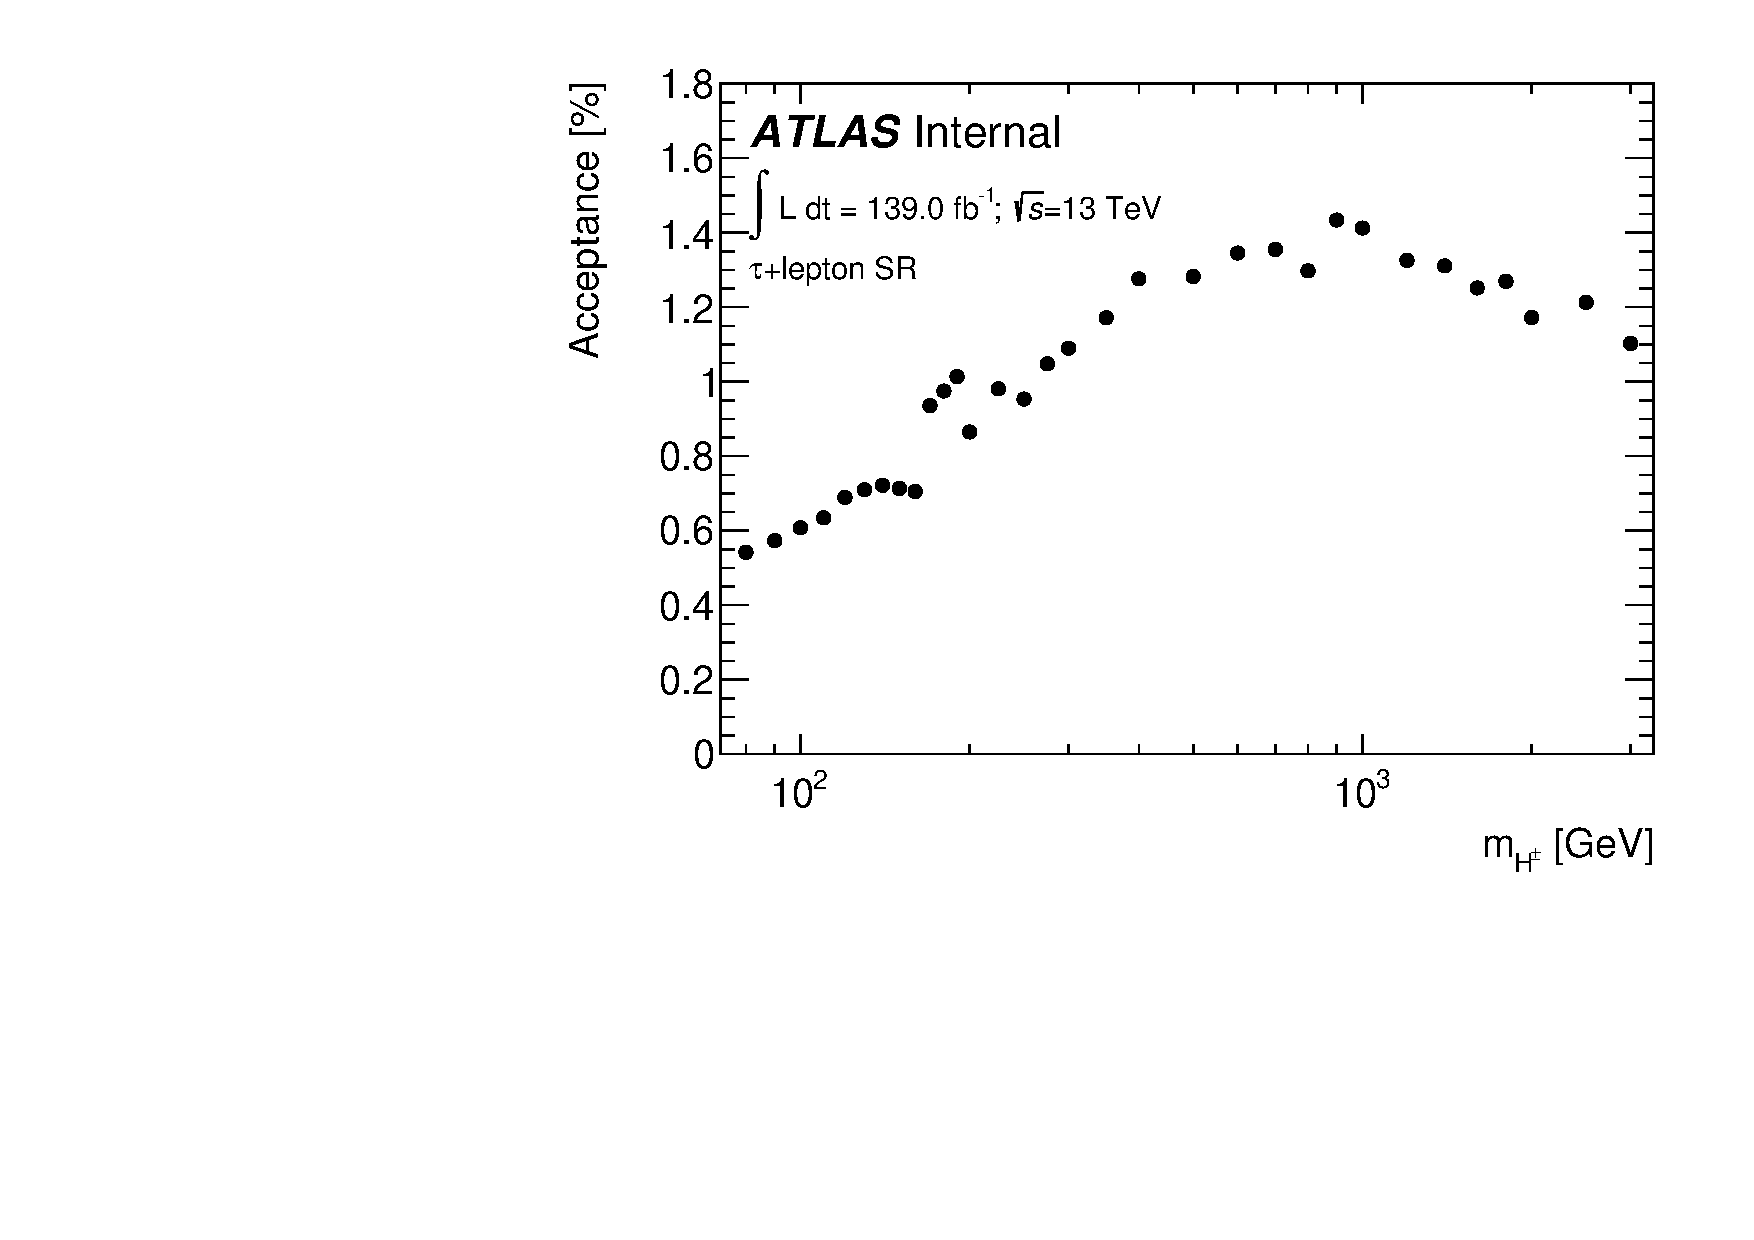
\includegraphics[width=0.5\textwidth]{chapters/chapter6_HPlus/images/Signal_Acceptance_Efficiency_SR_TAULEP.pdf}}
				\caption{\label{fig:signal-acceptance} Signal acceptance as a function of the charged Higgs boson mass for both the \taujets (a) and \taulep subchannels (b).}
			\end{figure}

	\section{Datasets}\label{sec:datasets}
		This analysis uses the full Run-2 ATLAS dataset collected between 2015 and 2018 corresponding to $139.0 \pm 2.4$ \ifb \cite{lumi-run2}. The datasets used are required to be included in the ATLAS ``Good Run Lists'' (GRLs), meaning they have passed nominal data quality checks with all detector subsystems operating within normal conditions. Further event cleaning is applied that removes events in which a reconstructed jet originated from detector noise or non-collision backgrounds. The collection of data throughout Run-2 can be seen in Figure \ref{fig:lhc-lumi}.

		\subsection{Signal Modeling}\label{ssec:sig-modeling}
		Monte Carlo (MC) simulations of \Hpm signal events are generated at varying orders dependent on \mHpm. In all cases, the 2HDM Type II model described in Section \ref{ssec:2HDM} is assumed and the generator MadGraph is used. The lower mass range corresponding to $\mHpm < 140$ GeV where a \Hpm takes the place of a $W^{\pm}$ in a top decay is generated at LO. The intermediate mass range of $140 \leq \mHpm < 200 $ GeV is generated at LO, taking into account the non-resonant, single-top resonant and double-resonant diagrams and their interferences. In this mass range, the final state contains one \Hpm, one $W^{\pm}$, and two b quark. For charged Higgs masses of 200 GeV and above, the \Hpm is produced in association with a top quark and is generated at NLO. In all cases, the parton generator is interfaced with Pythia 8 using the A14 underlying event tuning parameters \cite{Pythia8-tunes}. Table \ref{tab:signal-generated} shows the cross section and raw number of events generated for each \mHpm point for both subchannels.

		\begin{table}[!thp]
			\centering
			\resizebox{.65\textwidth}{!}{
			\begin{tabular}{| l | l | l | l |}
			\hline
			\mHpm [GeV] 	& $\sigma$ [pb] 	& \taulep Generated Events 	& \taujets Generated Events 	\\ \hline
			80 				& 61.639 			& 220k 						& 110k							\\
			90 				& 52.823 			& 220k 						& 110k							\\
			100 			& 43.777 			& 220k 						& 110k							\\
			110				& 34.770 			& 220k 						& 110k							\\
			120 			& 26.092 			& 220k 						& 110k							\\
			130 			& 18.069 			& 220k 						& 110k							\\ \hline
			140 			& 15.023 			& 220k 						& 220k							\\
			150 			& 7.681 			& 220k 						& 220k							\\
			160 			& 2.665 			& 220k 						& 220k							\\
			170 			& 0.63748 			& 220k 						& 220k							\\
			180 			& 0.52979 			& 220k 						& 220k							\\
			190 			& 0.47201 			& 220k 						& 220k							\\ \hline
			200 			& 0.55632 			& 110k 						& 220k							\\
			225 			& 0.44081 			& 110k 						& 220k							\\
			250 			& 0.3573 				& 110k 						& 220k							\\
			275 			& 0.28592 			& 110k 						& 220k							\\
			300 			& 0.23373 			& 110k 						& 220k							\\
			350 			& 0.15774 			& 110k 						& 220k							\\
			400 			& 0.10818 			& 110k 						& 220k							\\
			500 			& 0.054139 			& 110k 						& 220k							\\
			600 			& 0.02847 			& 110k 						& 220k							\\
			700 			& 0.015764 			& 110k 						& 220k							\\
			800 			& 0.009067 			& 110k 						& 220k							\\
			900 			& 0.005324 			& 110k 						& 220k							\\
			1000 			& 0.003271 			& 110k 						& 220k							\\
			1200 			& 0.001311 			& 110k 						& 220k							\\
			1400 			& 0.000558 			& 110k 						& 220k							\\
			1600 			& 0.000252 			& 110k 						& 220k							\\
			1800 			& 0.000120 			& 110k 						& 220k							\\
			2000 			& 0.0000587 		& 110k 						& 220k							\\
			2500 			& 0.0000111			& 110k 						& 220k							\\
			3000 			& 0.00000234		& 110k 						& 220k							\\ \hline
			\end{tabular}}
			\caption{For each \Hpm mass the generator xcross-section $(\sigma \times BR(\HpmLong))$ is given, as well as the number of generated events for both \taulep and \taujets subchannels.}
			\label{tab:signal-generated}
		\end{table}
		% \pagebreak

	\section{Background Modeling}\label{sec:bkg-modeling}
		The main sources of backgrounds are shown in Table \ref{tab:backgrounds}, separated between backgrounds with a prompt \tauhad in the hard scatter process and those that arise from the misidentification of other physics objects as a \tauhad. The cross section of all simulated background samples and the relevant generators can be seen in Table \ref{tab:bkg-xs}. Control regions that are designed to be orthogonal to the signal region are created for both subchannels in order to study the modeling of the backgrounds. These control regions are defined by the cuts in Table \ref{tab:taujet-control-regions} (\taujets) and Table \ref{tab:taulep-control-regions} (\taulep). For the \taulep subchannel the Same Sign and b-veto control regions are further split into two control regions, one that requires a $\mu$ in the event and another that requires an electron. 

		

    \begin{table}[!thp]
      \centering
      \resizebox{\textwidth}{!}{
      \begin{tabular}{| l | l |}
      \hline
      Backgrounds w/ prompt \tauhad & Backgrounds w/ fake $\tau$ \\
      \hline \hline
      $t\bar{t}$ estimated with MC       & Fake $j \to \tau$ estimated with data driven fake factor method \\ \hline
      $W(Z)+jets$ estimated with MC         & Fake $\ell \to \tau$ estimated with MC, validated on $Z \to ee$\\ \hline
      Diboson estimated with MC & \\
      \hline
      \end{tabular}}
      \caption{Dominant backgrounds from prompt \tauhad and fake \tauhad candidates.}
      \label{tab:backgrounds}
    \end{table}

		\begin{table}[!thp]
			\begin{center}
			\small
			\resizebox{0.5\textwidth}{!}{
			\begin{tabular}{|c||c|c|}
			\hline
			Background process & Generator \& & Cross section \\
			  & parton shower & number(s) [pb] \\
			\hline \hline
			$\begin{array}{c}
			$\ttbar$~\mbox{with at least one lepton $\ell$} \\ 
			\end{array}$ &
			$\begin{array}{c}
			\mbox{{\textsc Powheg}}~\& \\
			\mbox{{\textsc Pythia8}}
			\end{array}$
			& 729.77* \\
			\hline
			$\begin{array}{c}
			\mbox{Single top-quark}\\ 
			\mbox{$t$-channel}
			\end{array}$ & & 59.17* \\
			$\begin{array}{c}
			\mbox{Single top-quark}\\ 
			\mbox{$s$-channel}
			\end{array}$ &
			$\begin{array}{c}
			\mbox{{\textsc Powheg}}~\& \\
			\mbox{{\textsc Pythia8}}
			\end{array}$ & 3.29* \\
			$\begin{array}{c}
			\mbox{Single top-quark}\\ 
			\mbox{$Wt$-channel}
			\end{array}$  & & 83.83  \\
			\hline
			$\begin{array}{c}
			~ \\
			W(\ell\nu) + \mbox{jets} \\ 
			~ \\
			\end{array}$ &
			$\begin{array}{c}
			~ \\
			\mbox{Sherpa 2.2.1} \\ 
			~ \\
			\end{array}$ &
			$\begin{array}{c}
			2.0\times 10^4 \\
			2.0\times 10^4 \\ 
			2.0\times 10^4 \\
			\end{array}$ \\
			\hline
			$\begin{array}{c}
			Z/\gamma^{\ast}(\ell\ell,\nu\nu) + \mbox{jets} \\
			\end{array}$ & 
			$\begin{array}{c}
			~ \\
			\mbox{Sherpa 2.2.1} \\ 
			~ \\
			\end{array}$  &
			$\begin{array}{c}
			2.1 \times 10^3  \\
			2.1 \times 10^3  \\ 
			2.1 \times 10^3  \\
			\end{array}$ \\

			\hline
			$WW$  &  & 54.81 \\
			$WZ$  &  $\begin{array}{c}
			\mbox{{\textsc Powheg}}~\& \\
			\mbox{{\textsc Pythia8}}
			\end{array}$ & 16.34 \\
			$ZZ$  &  & 8.94 \\
			\hline
			\end{tabular}}
			\normalsize
			\caption{\label{tab:bkg-xs}
			Cross sections for the main SM 
			background samples at \sqs. 
			Here, $\ell$ refers to the three lepton families $e$, $\mu$ and 
			$\tau$. All background cross sections are normalized to NNLO predictions, 
			except for diboson events, where the NLO prediction is used. A '*' indicates
			that the quoted cross section for the sample is neglecting leptonic/hadronic
			branching ratios.
			}
			\end{center}
		\end{table}

		\begin{table}[!thp]
			\begin{subtable}[c]{0.45\textwidth}
				\centering
				\begin{tabular}{| c |}
					\hline
        	\textbf{\ttbar Control Region} \\ \hline \hline
          1 \tauhad \\
          $\pt^{\tau} > 40 $ GeV \\
          $\geq 3 $ jets\\
          $\geq 2 $ \bjets\\
          $\Etm > 150 GeV$ \\
          $m_{T}(\tau, \Etm) < 100 \: GeV$ \\
          \hline
				\end{tabular}
				\subcaption{\ttbar modeling}
			\end{subtable}
			\begin{subtable}[c]{.45\textwidth}
				\centering
				\begin{tabular}{| c |}
					\hline
					\textbf{b-veto Control Region} \\ \hline \hline
					1 \tauhad \\
					$\pt^{\tau} > 40 \: GeV $  \\
					$\geq 3$ jets\\
					% $n\_bjets > 2$ \\
					$\pt^{jet} > 25 \: GeV$ \\
					$\Etm > 150 GeV$ \\
					$m_{T}(\tau, \Etm) > 50 \: GeV$ \\
					b veto \\
					$\ell$ veto \\
					\hline
				\end{tabular}
				\subcaption{Close to signal region}
			\end{subtable}
			\begin{subtable}[c]{.45\textwidth}
				\centering
				\begin{tabular}{| c |}
					\hline
					\textbf{W+Jets Control Region} \\ \hline \hline
					1 \tauhad \\
					$\pt^{\tau} > 40 \: GeV $  \\
					$\geq 3$ jets \\
					$\pt^{jet} > 25 \: GeV$ \\
					$\Etm > 150 GeV$ \\
					$m_{T}(\tau, \Etm) > 100 \: GeV$ \\ 
					b veto \\
					$\ell$ veto \\
					\hline
				\end{tabular}
				\subcaption{W+Jets modeling}
			\end{subtable}
			\begin{subtable}[c]{.45\textwidth}
				\centering
				\begin{tabular}{| c |}
					\hline
					\textbf{b-veto $m_{T}\geq100$ Control Region} \\ \hline \hline
					1 \tauhad \\
					$\pt^{\tau} > 40 \: GeV $  \\
					$\geq 3$ jets \\
					$\pt^{jet} > 25 \: GeV$ \\
					$\Etm > 150 GeV$ \\
					$m_{T}(\tau, \Etm) > 100 \: GeV$ \\
					b veto \\
					$\ell$ veto \\
					\hline
				\end{tabular}
				\subcaption{Fake $j \to \tau$ enriched region}
			\end{subtable}

			\caption{Control region definitions for the \taujets subchannel.}
			\label{tab:taujet-control-regions}
		\end{table}

		\begin{table}[!thp]
			\begin{subtable}[c]{0.45\textwidth}
				\centering
				\begin{tabular}{| c |}
					\hline
        	\textbf{Dilepton-btag CR} \\ \hline \hline
          $\tau$ veto \\
          $n\geq 1$ jets \\
          $\pt^{jet} > 25 GeV$ \\
          $\geq 1$ \bjets \\
          $\Etm > 50 GeV$ \\
          1 $e$ \\
          1 $\mu$ \\
          \hline
				\end{tabular}
				\subcaption{\ttbar and single top modeling}
			\end{subtable}
			\begin{subtable}[c]{.45\textwidth}
				\centering
				\begin{tabular}{| c |}
					\hline
	        \textbf{b-veto CR} \\ \hline \hline
          1 \tauhad \\
          $\pt^{\tau} > 30 \: GeV $  \\
          1 $e (\mu) $ \\
          Veto $\mu \:(e)$ \\
          Opposite sign $\tau$ $e \: (\mu)$ \\
          $\geq 1$ jets  \\
          $\pt^{jet} > 25 GeV$ \\
          $\Etm > 50 GeV$ \\
          1 tight $e \: (\mu)$ \\
          \hline					
				\end{tabular}
				\subcaption{Close to signal region}
			\end{subtable}
			\begin{subtable}[c]{.45\textwidth}
				\centering
				\begin{tabular}{| c |}
					\hline
        	\textbf{Zee CR} \\ \hline \hline
          1 \tauhad \\
          $\pt^{\tau} > 30 \: GeV $  \\
          veto $\mu$ \\
          Opposite sign $\tau$ $e$ \\
          $\geq 1$ jets \\
          $\pt^{jet} > 25 GeV$ \\
          \bjet veto \\
          $\Etm > 50 GeV$ \\
          1 $e$\\
          $40 < mass(\tau,e) < 140 GeV$ \\
          \hline
				\end{tabular}
				\subcaption{Fake $\ell \to \tau$ enriched region}
			\end{subtable}
			\begin{subtable}[c]{.45\textwidth}
				\centering
				\begin{tabular}{| c |}
					\hline
	        \textbf{Same Sign CR} \\ \hline \hline
          1 \tauhad \\
          $\pt^{\tau} > 30 \: GeV $  \\
          Same sign $\tau \: e(\mu)$ \\
          Veto $\mu\:(e)$ \\
          $\geq 1 jets$ \\
          $\pt^{jet} > 25 GeV$ \\
          $\Etm > 50 GeV$  \\
          1 tight $e \: (\mu)$ \\
          \hline
				\end{tabular}
				\subcaption{Fake $j \to \tau$ enriched region}
			\end{subtable}

			\caption{Control region definitions for the \taulep subchannel.}
			\label{tab:taulep-control-regions}
		\end{table}

		As seen in Table \ref{tab:backgrounds} misidentified objects appearing as \tauhad candidates comprise a significant portion of the total background. Fakes arising from $\ell \to \tau$ misidentification are well modeled in MC simulations and are reweighted with scale factors provided by the ATLAS $\tau$ combined performance group. The mass of the \tauhad electron system can be seen in Figure \ref{fig:zee-mass} as verification of fake $\ell \to \tau$ modeling. However, fakes due to $j \to \tau$ misidentification are not well modeled in MC simulations due to a poor misunderstanding of systematic uncertainties associated with the fake \tauhad object and limited statistics of simulated events. Instead, a data driven method is used to extract a scaling constant referred to as a fake factor.

		\begin{figure}[!thp]
			\centering
			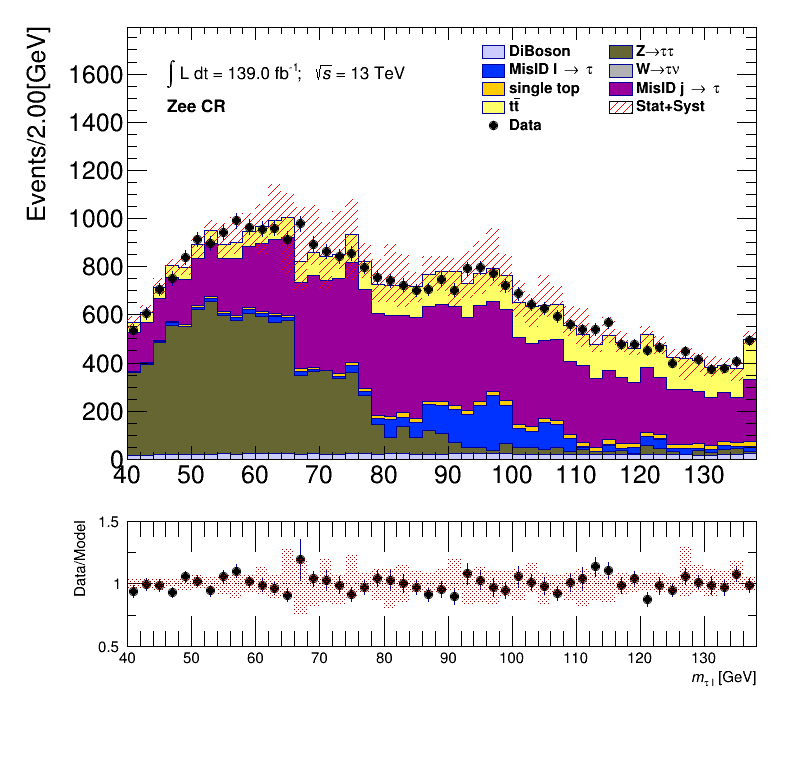
\includegraphics[width=.5\textwidth,keepaspectratio=true]{chapters/chapter6_HPlus/images/taulep/tau_0_lep_0_mass_ZEE.png}
			\caption{Mass of $\tau$ - e system in the Zee control region.}
			\label{fig:zee-mass}
		\end{figure}

		In the \taulep final state a significant portion of $j \to \tau$ fakes come from misidentifying \tauhad candidates in W+Jets events that contain a true $\ell$ in the W decay and have a misidentified jet as a \tauhad. Fakes of this manner also arise from QCD-like multi-jet interactions. The fake factor method used to estimate the amount of expected fake \tauhad objects that pass the \tauhad identification procedure described in Section \ref{ssec:reco-tau}. This method applies weights, or fake factors, to a subset of "anti-\tauhad" objects that have failed the selection and identification criteria in the signal region. A control region is defined to be rich in anti-\tauhad objects, where the \tauhad candidates fail the loose $\tau$ working point but have a $\tau$ identification RNN score of greater than 0.01. The fake factor and number of events with misidentified \tauhad objects $(N_{\tau})$ are defined as:
		\begin{equation}\label{eqn:ff}\begin{split}
		FF = \frac{ N^{\tau-id} }{N^{anti-\tau-id}} \\
		N_{fakes}^{\tau} = N^{anti-\tau}_{fakes} \times FF
		\end{split}\end{equation}
		Both of these values are then corrected for \tauhad candidates matching a true hadronic $\tau$ at generator level:
		\begin{equation}\label{eqn:ff-corrected}\begin{split}
		N^{\tau-id} = N^{\tau-id}(Data) - N^{\tau-id}(MC) \\
		N^{anti-\tau}_{fakes} = N^{anti-\tau}(Data) - N^{anti-\tau}_{true} (MC)
		\end{split}\end{equation}
		Two control regions are created, one to capture the multi-jet (MJ) fakes and the other to study the W+jets fakes. The MJ control region uses the \taujets signal region definition with an additional b-veto and an $\Etm < 80$ GeV cut. The W+jets control region uses the \taulep signal region definition with a b-veto, no \Etm cut, and a cut on the transverse mass of the $\ell$-\Etm system of $60 < m_{T}(\ell, \Etm)<160$ GeV.
		The FF in the signal region is defined as 
		\begin{equation}\label{eqn:ff-sig}
		FF_{sig} = \alpha_{MJ} \times FF_{MJ} + (1 - \alpha_{MJ}) \times FF_{W+jets}
		\end{equation}
		where $\alpha$ is taken from a template fit of the $\tau$-ID score distributions of the anti-$\tau$s using template shapes from the anti-$\tau$ distributions in the MJ and W+jets control regions. In the signal regions, the number of events containing fake-\tauhad candidates is defined as
		\begin{equation}\label{eqn:nfakethad}
			N_{fake-\tau} = FF_{sig} \times N_{anti-\tau} 
		\end{equation}
		Figure \ref{fig:FF_COM} shows FF plotted in each control region for 1-prong and 3-prong \tauhad binned in $\pt{\tau}$; extracted $\alpha$ values and their fits can be seen in Appendix \ref{app:fake-factors}.
		\begin{figure}[h!]
		  \begin{center}
		    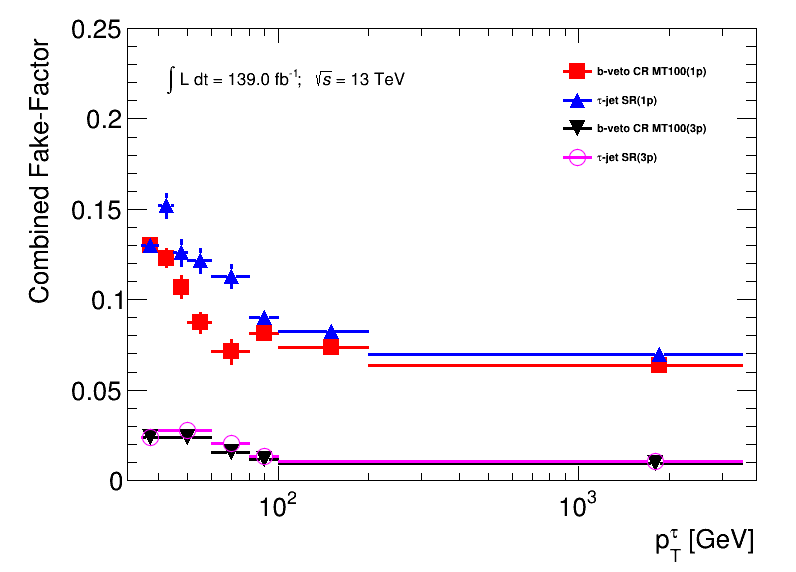
\includegraphics[width=0.45\textwidth]{chapters/chapter6_HPlus/images/FFs/FFs_COM_inclusive__taujet.png} \qquad
		    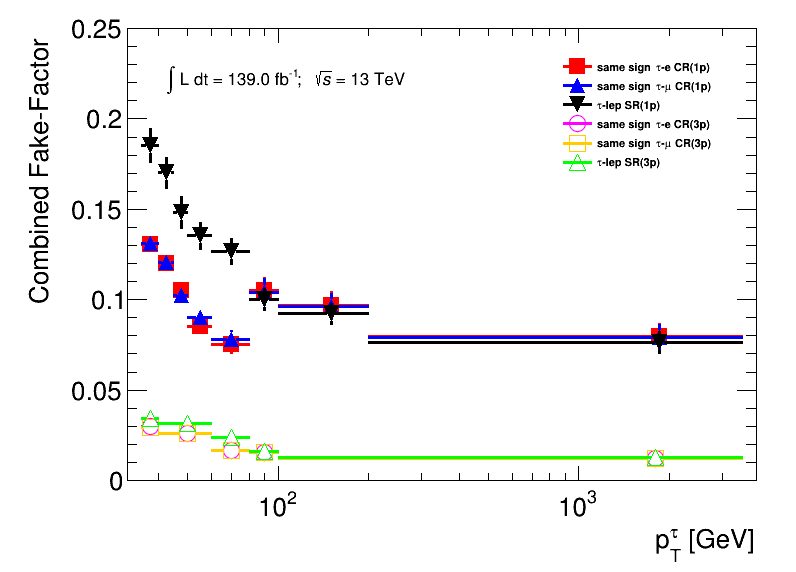
\includegraphics[width=0.45\textwidth]{chapters/chapter6_HPlus/images/FFs/FFs_COM_inclusive__taulep.png} 
		  \end{center}
		  \caption{
		Combined fake factors for the \taujets b-veto $\mathrm{m_{T}}>$100 control region, \taujets signal region, $\tau$+electron(muon) with same-sign control region and the \taulep signal region. Error bars represent systematic uncertainties of the method. 
		}
		  \label{fig:FF_COM}
		\end{figure}


		To verify background modeling, the \Etm distributions in each of the control regions are plotted with final scale factors including fake factors in Figure \ref{fig:bkg-met-taujets} (\taujets) and Figure \ref{fig:bkg-met-taulep} (\taulep). These plots include a ratio of reconstructed data events and simulated MC events bin by bin to ensure proper modeling across variable shapes. More background modeling plots can be seen in Appendix \ref{app:valid-plots}.

		\begin{figure}[!thp]
			\begin{center}    
			% 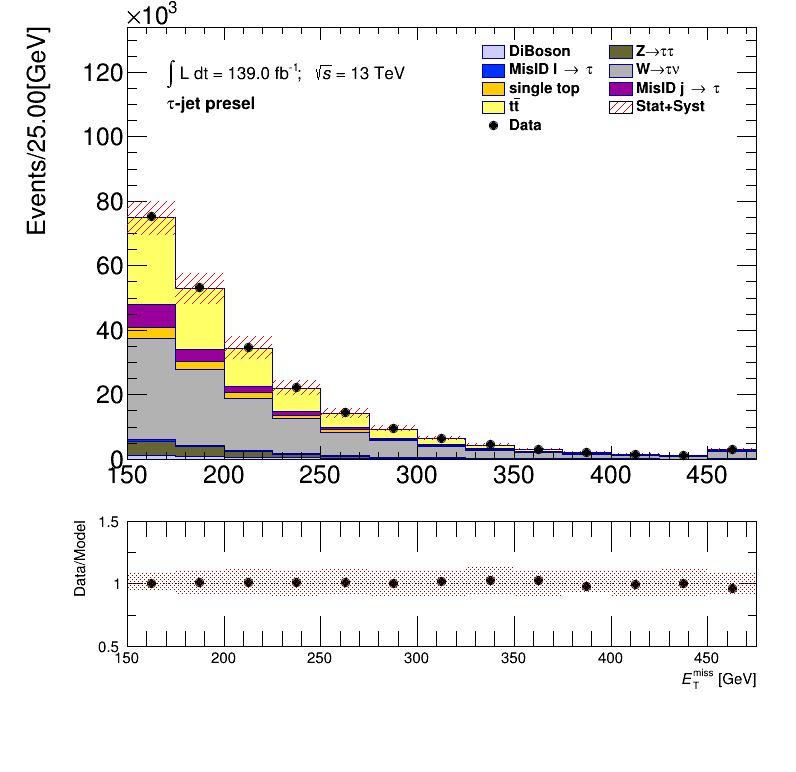
\includegraphics[width=0.45\textwidth]{chapters/chapter6_HPlus/images/taujets/met_et_TAUJET_PRESEL.png} \\
			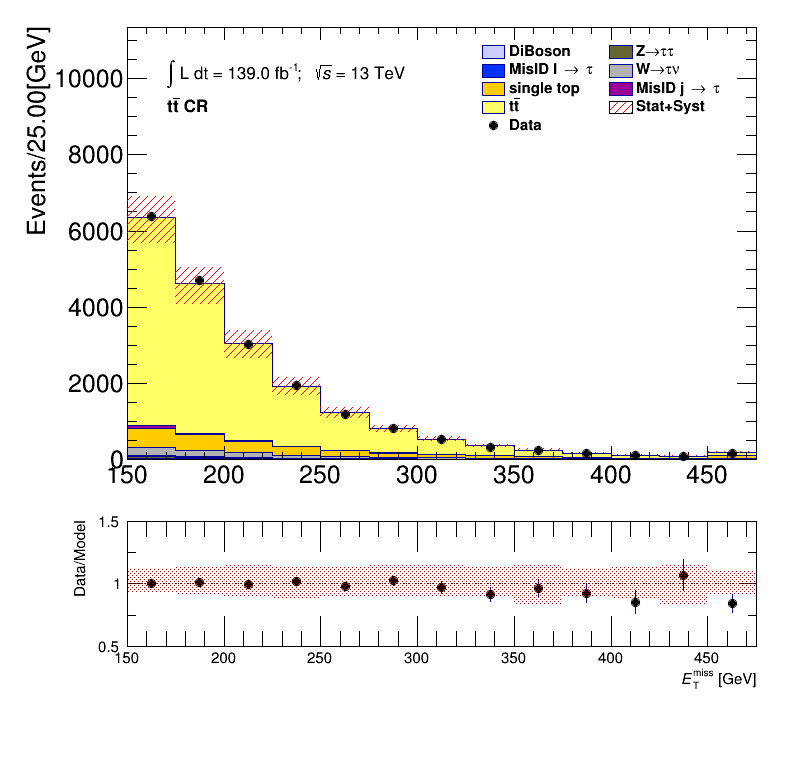
\includegraphics[width=0.45\textwidth]{chapters/chapter6_HPlus/images/taujets/met_et_TTBAR.png}
			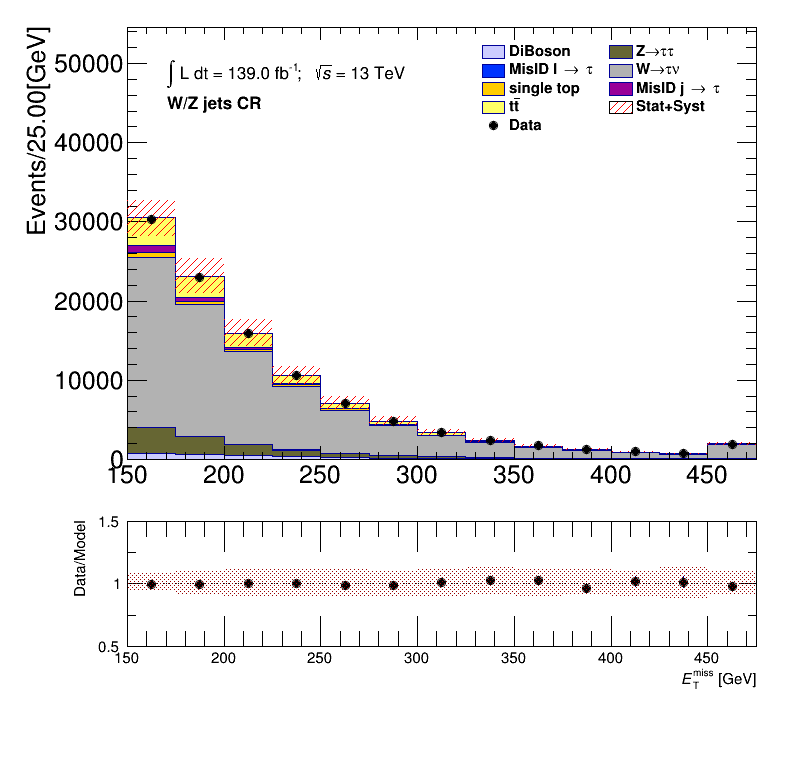
\includegraphics[width=0.45\textwidth]{chapters/chapter6_HPlus/images/taujets/met_et_WJETS.png} \\
			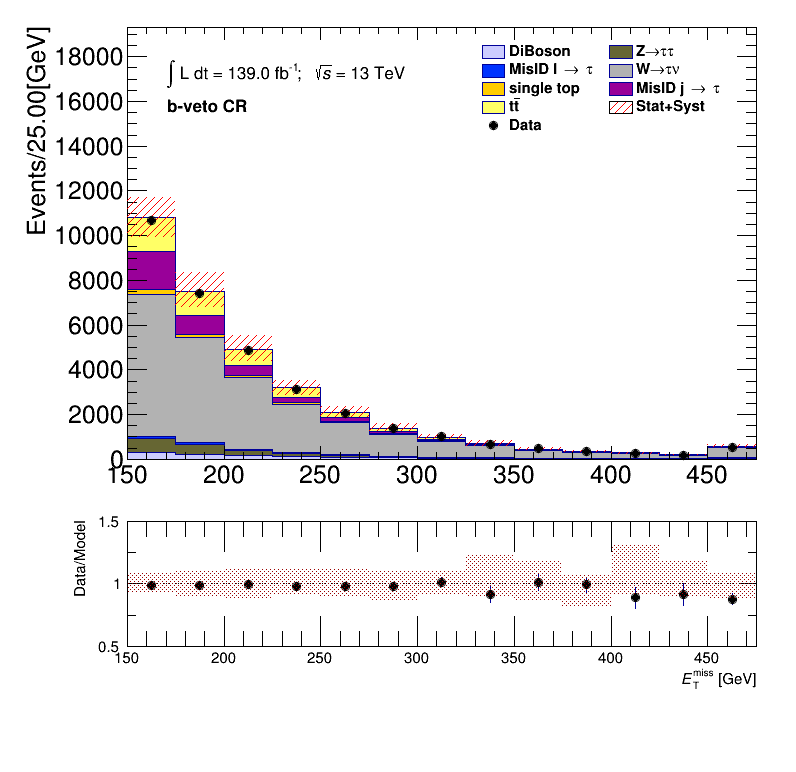
\includegraphics[width=0.45\textwidth]{chapters/chapter6_HPlus/images/taujets/met_et_BVETO.png}
			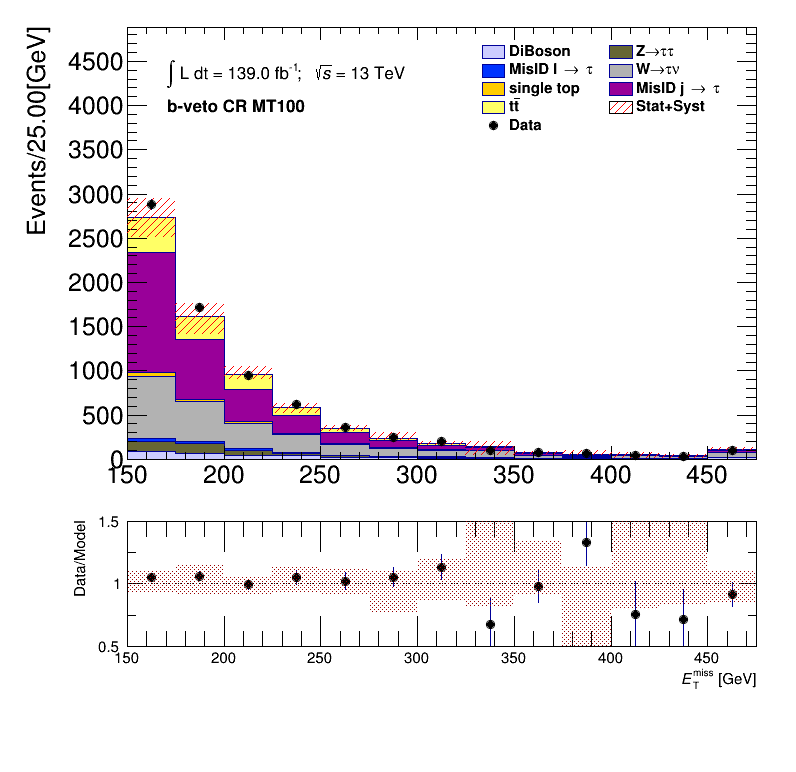
\includegraphics[width=0.45\textwidth]{chapters/chapter6_HPlus/images/taujets/met_et_BVETO_MT100.png} \\
			\end{center}
			\caption{
			Comparison between the predicted and the measured \Etm distributions in various control regions defined for the \taujets channel. The uncertainty band includes both statistical and systematic uncertainties on the background prediction. 
			}
			\label{fig:bkg-met-taujets}
		\end{figure}

		\begin{figure}[!thp]
			\begin{center}    
			% 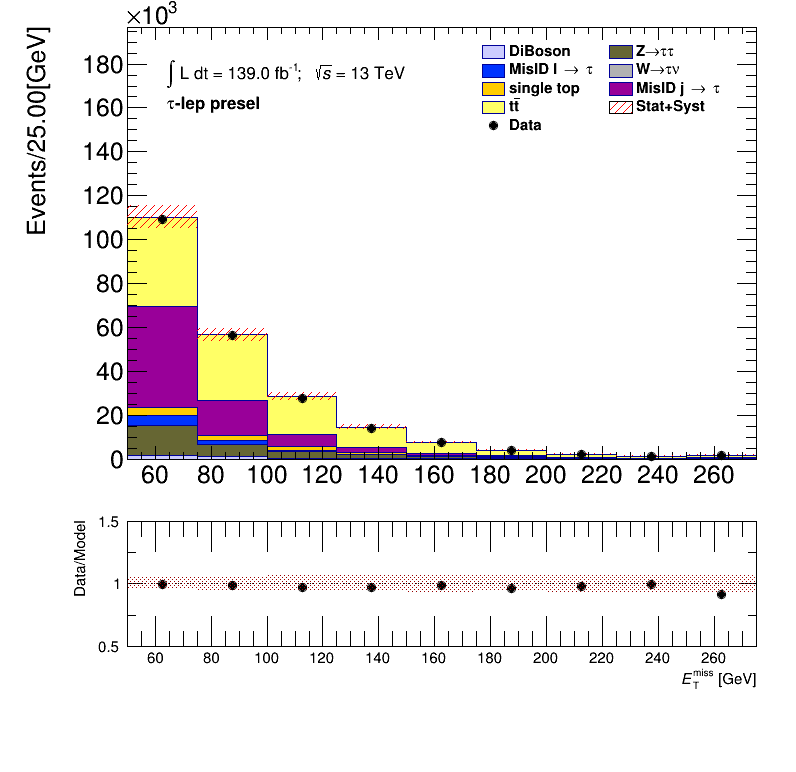
\includegraphics[width=0.45\textwidth]{chapters/chapter6_HPlus/images/taulep/met_et_TAULEP_PRESEL.png} \\
			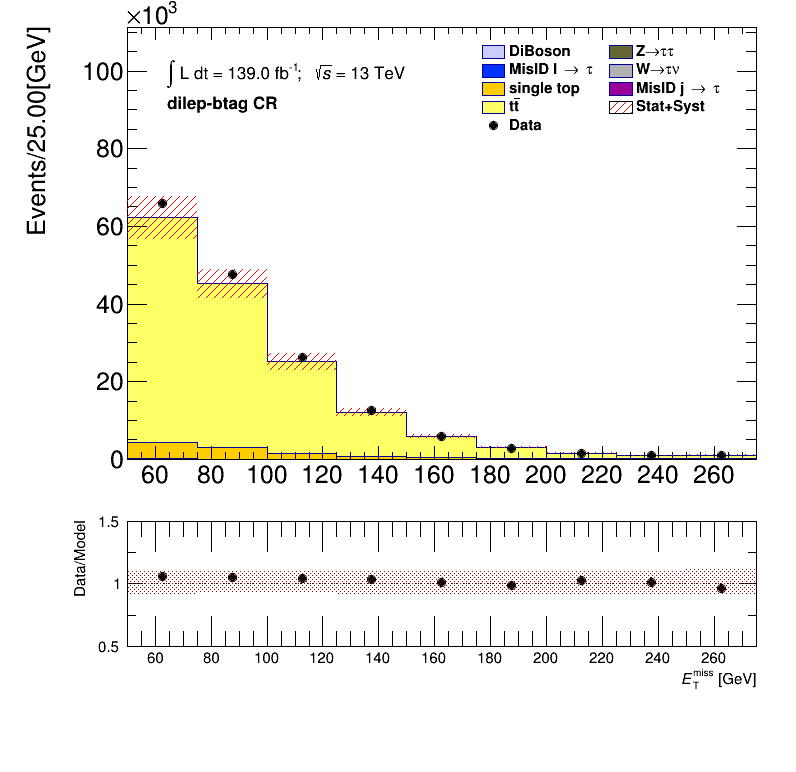
\includegraphics[width=0.45\textwidth]{chapters/chapter6_HPlus/images/taulep/met_et_DILEP_BTAG.png}
			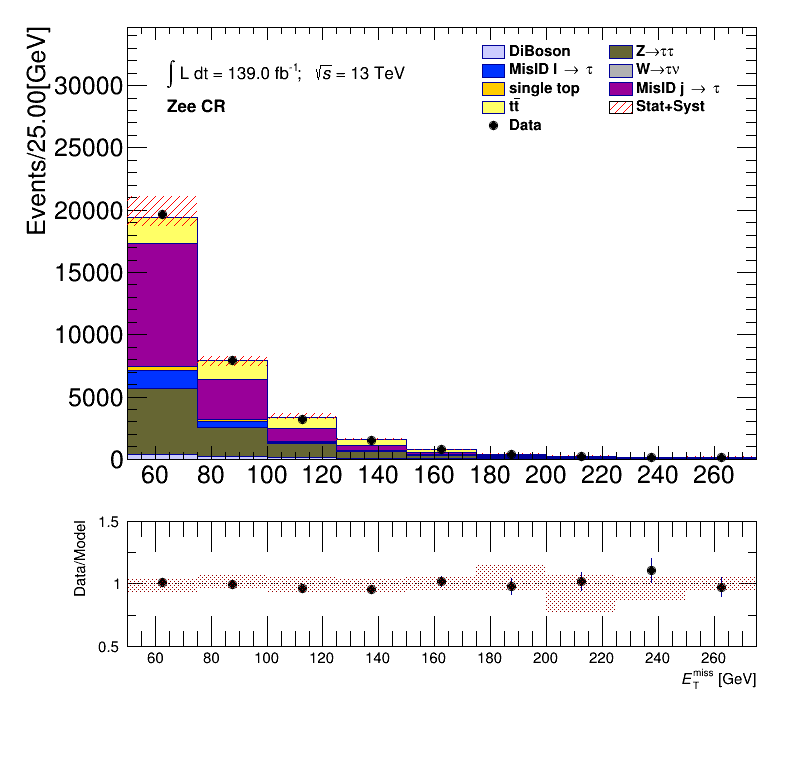
\includegraphics[width=0.45\textwidth]{chapters/chapter6_HPlus/images/taulep/met_et_ZEE.png} \\
			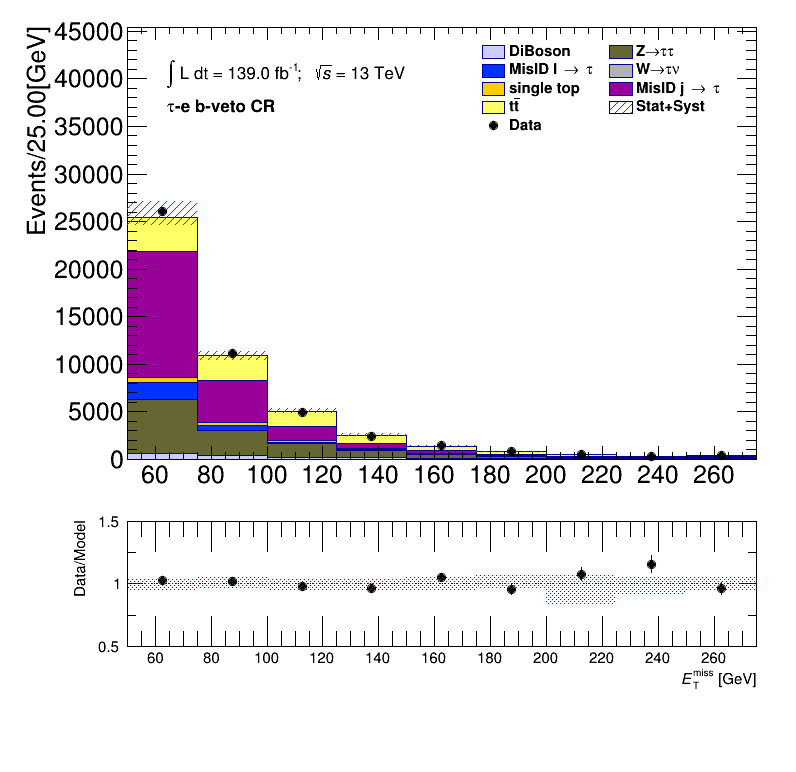
\includegraphics[width=0.45\textwidth]{chapters/chapter6_HPlus/images/taulep/met_et_TAUEL_BVETO.png} 
			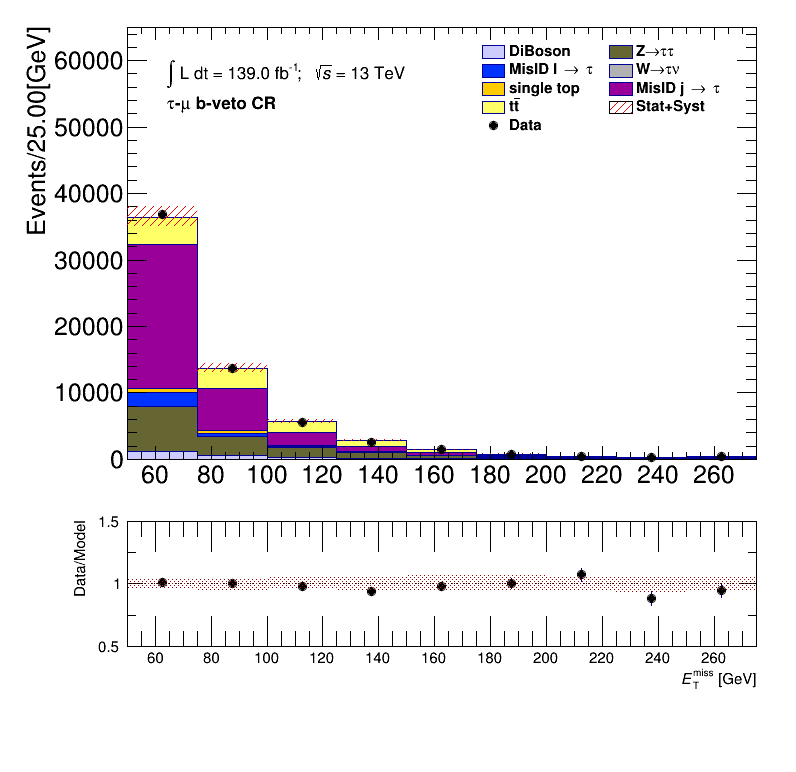
\includegraphics[width=0.45\textwidth]{chapters/chapter6_HPlus/images/taulep/met_et_TAUMU_BVETO.png} \\
			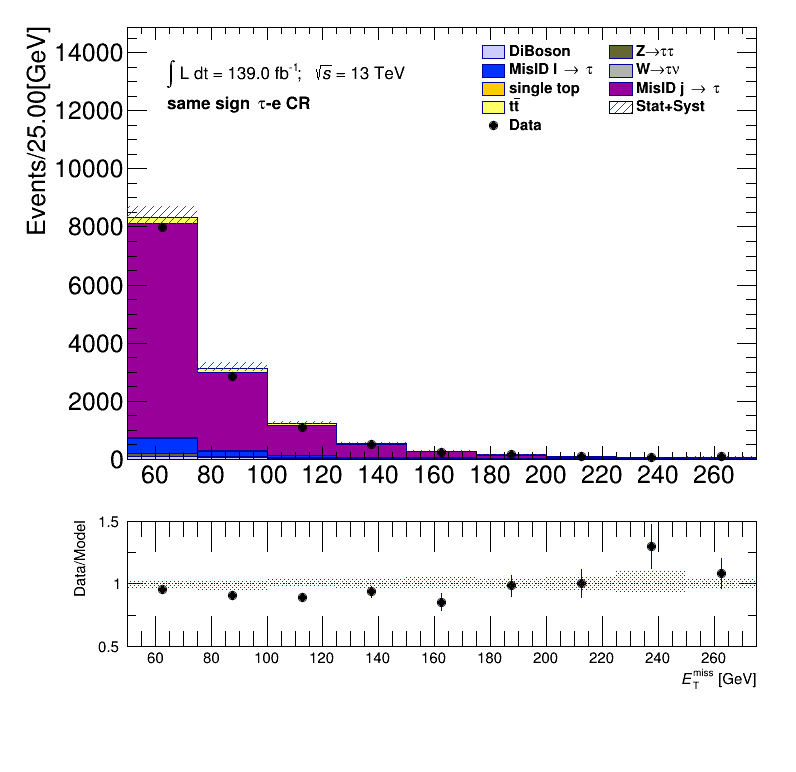
\includegraphics[width=0.45\textwidth]{chapters/chapter6_HPlus/images/taulep/met_et_SS_TAUEL.png} 
			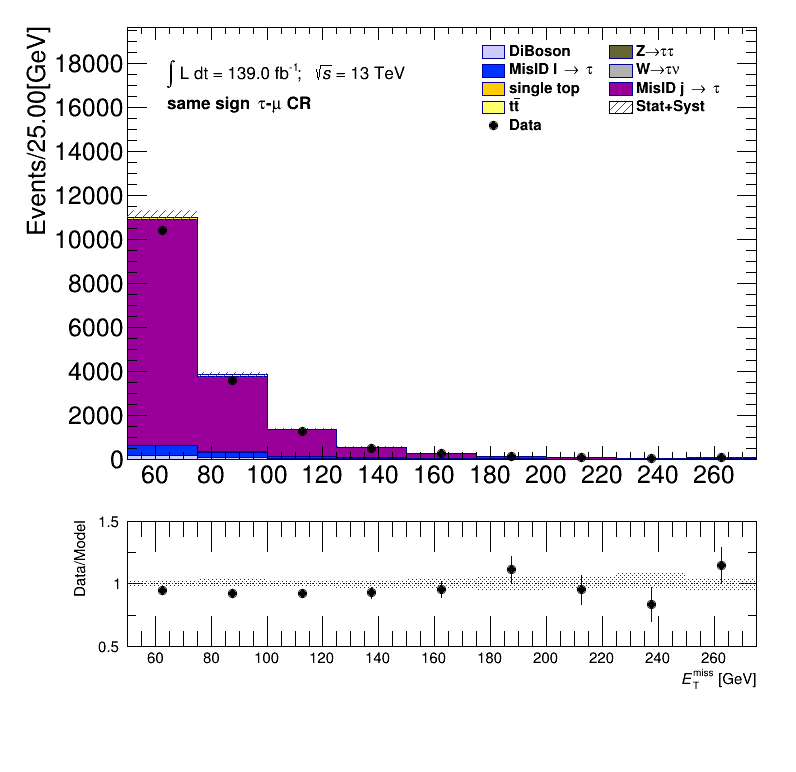
\includegraphics[width=0.45\textwidth]{chapters/chapter6_HPlus/images/taulep/met_et_SS_TAUMU.png} \\
			\end{center}
			\caption{
			Comparison between the predicted and the measured \Etm distributions in various control regions defined for the \taulep channel. The uncertainty band includes both statistical and systematic uncertainties on the background prediction. 
			}
			\label{fig:bkg-met-taulep}
		\end{figure}

	\clearpage
	\section{Multivariate Analysis Techniques}\label{sec:mva}
		Once variables distributions are properly scaled and data/MC agreement is verified, multivariate analysis techniques are employed to separate signal-like events from background-like events in the signal regions. In the previous publication (described in Section \ref{ssec:Prev Hpm}), BDTs binned in \mHpm were used as the classifier, this publication use one PNN for the entire \mHpm spectrum. BDTs excel at separating linear correlations, whereas neural networks take advantage of nonlinear correlations. In the case of a PNN the parameterized variable, here \mHpm, is taken as an input to the network in addition with other input variables. PNNs offer the advantage of having one classifier model that can evaluate at any \mHpm value by learning how the signal event topology changes as \mHpm varies \cite{PNN}. For illustrative purposes, expected limits on $\sigma(\pp\to tb\Hpm)\times \mathrm{\cal{B}}(\Hpm \to \tau \nu)$ in both subchannels is shown comparing an optimized BDT and an unoptimized PNN in Figure \ref{fig:bdt-vs-pnn-expected-limits}. It is seen that the PNN performs similarly to the BDTs used in the previous analysis. A PNN was chosen as the discriminator. 

		\begin{figure}
		\subfloat[\label{fig:bdt-vs-pnn-expected-limits-a}]{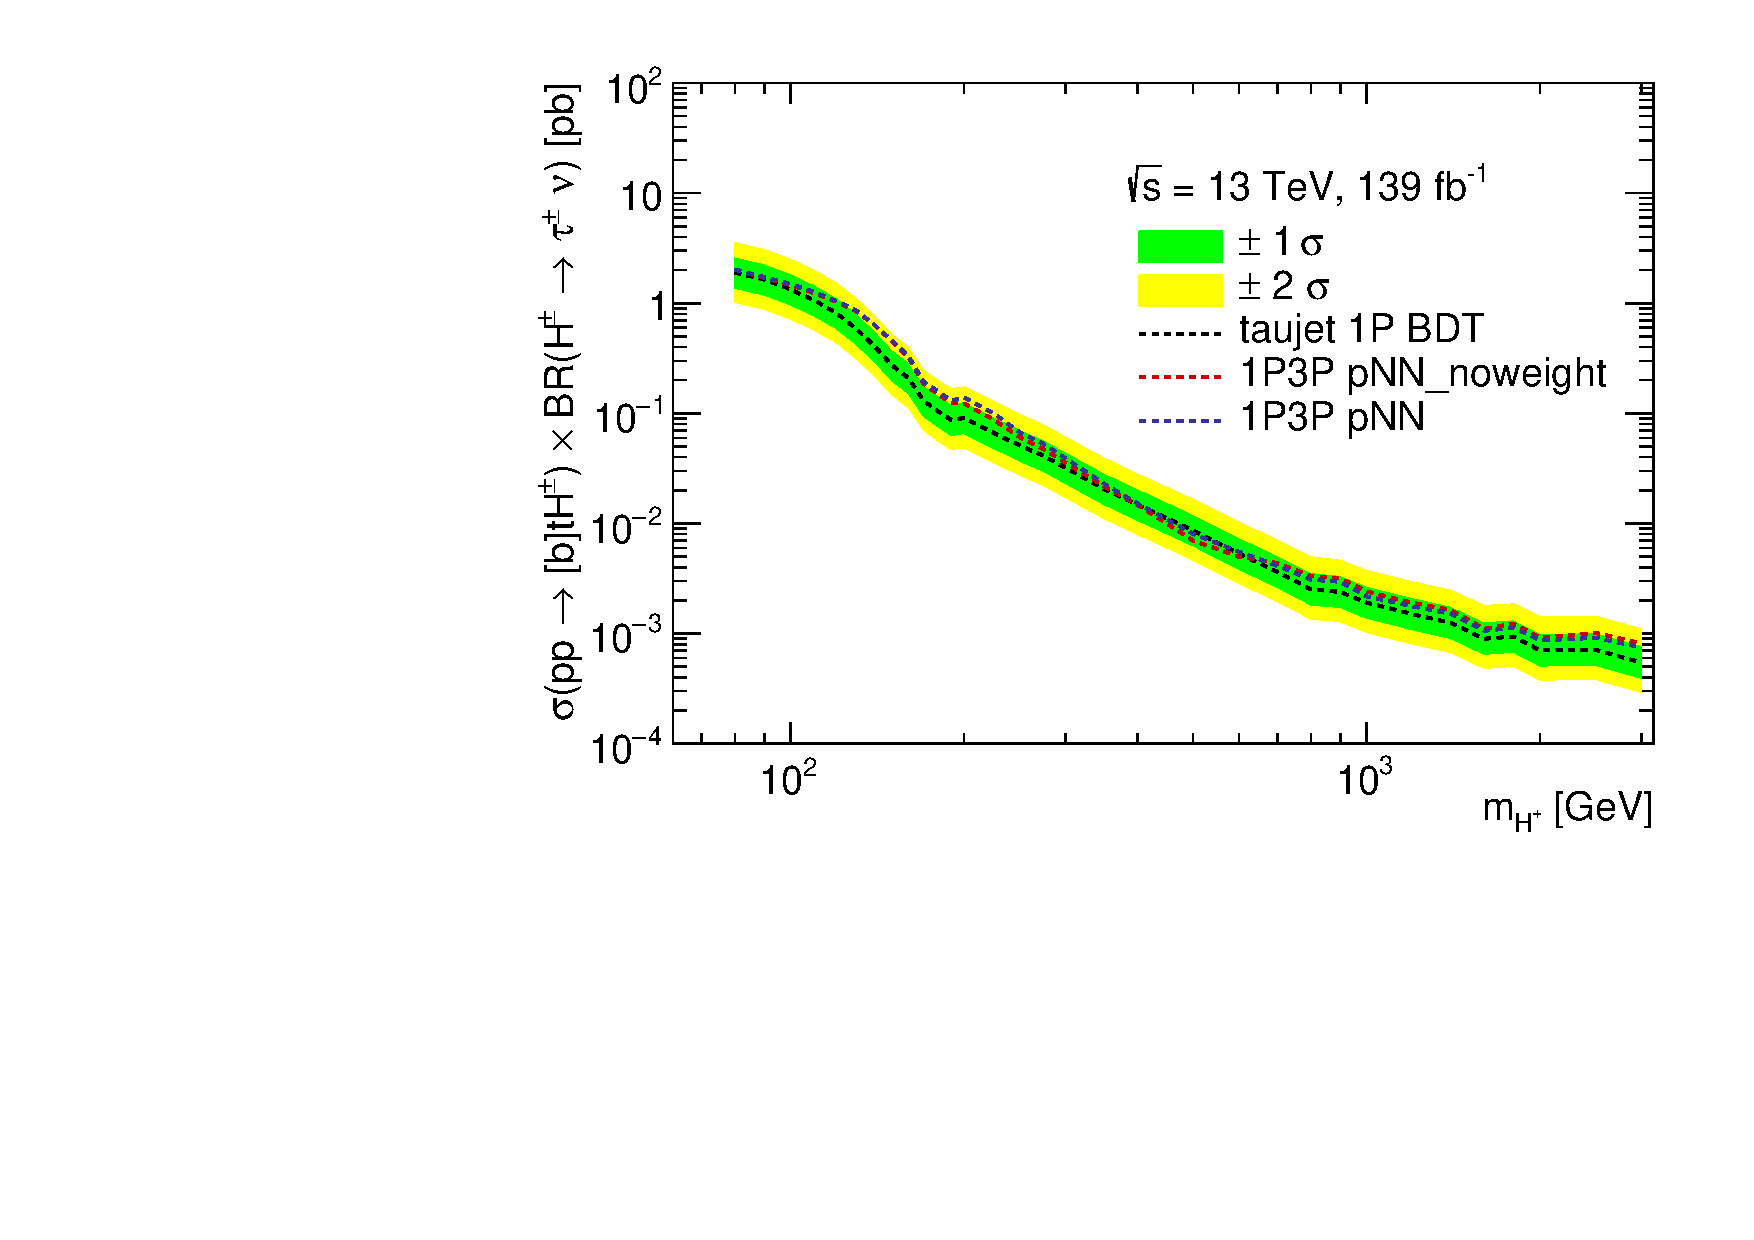
\includegraphics[width=.5\textwidth]{chapters/chapter6_HPlus/images/Limits/exp_limit_log_taujet.pdf}}
		\subfloat[\label{fig:bdt-vs-pnn-expected-limits-b}]{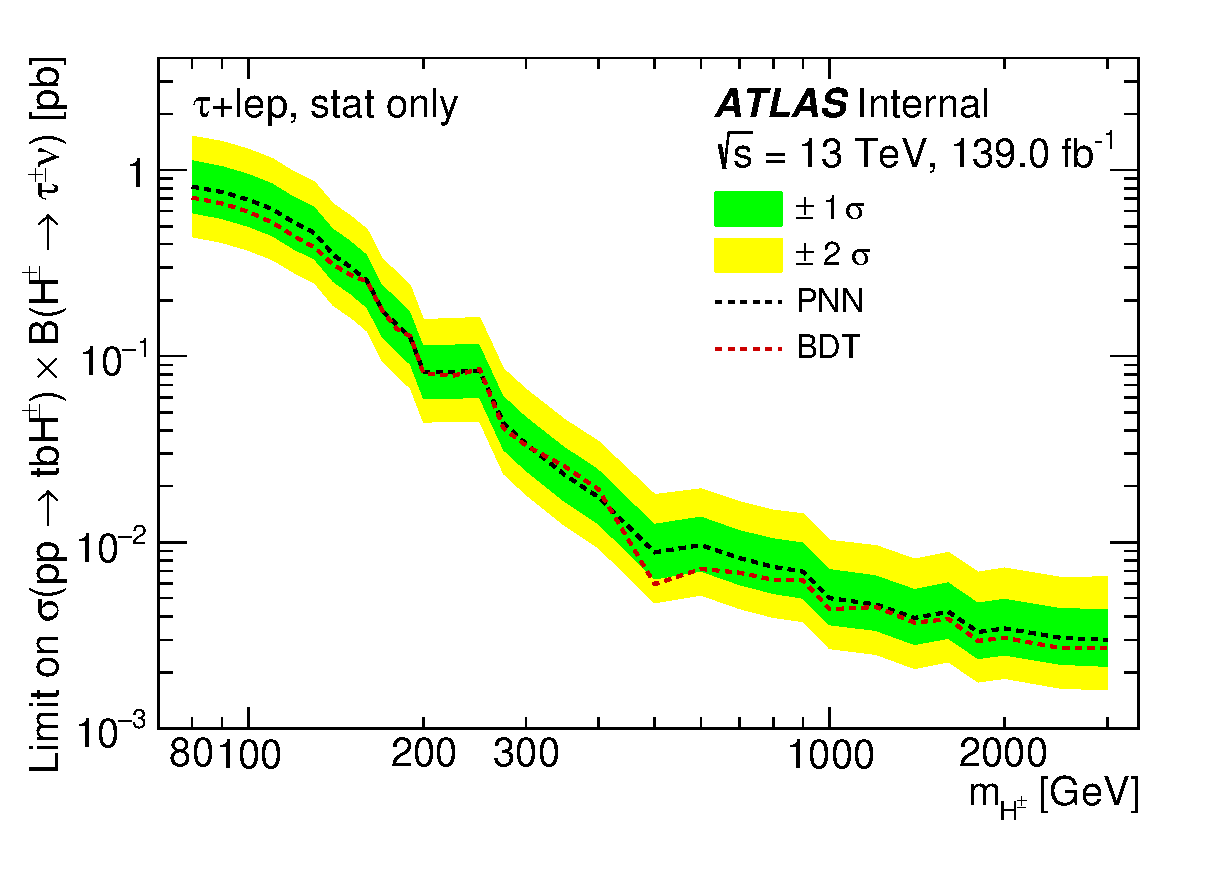
\includegraphics[width=.5\textwidth]{chapters/chapter6_HPlus/images/Limits/Exp_Limit_log_taulep.eps}}
		\caption{Comparison of performance of an optimized BDT and an unopitmized PNN on expected limits on $\sigma(\pp\to tb\Hpm)\times \mathrm{\cal{B}}(\Hpm \to \tau \nu)$ in the \taujets (a) and \taulep (b) signal regions. }
		\label{fig:bdt-vs-pnn-expected-limits}
		\end{figure}

		A neural network (NN) is a computing system loosely inspired by the human brain. NNs combine adaptive nonlinear basis functions in an attempt to perform a task, classification in the context of this dissertation. A NN contains layers of nodes connected to each other with an associated weight and threshold. As long as a node has output greater than the given threshold value, data will flow through that node. Otherwise, that node is not activated and data are not sent to the next layer. The NN as a whole relies on a process called training where the node weights are varied, an accuracy is calculated based on a given loss function, the weights are then varied again and the process repeats. This is done until a preferred accuracy is reached; the final node weights are saved and new data can be evaluated. A diagram of a PNN can be seen in Figure \ref{fig:PNN-diagram}, where the parameterized input is labeled as $\theta$. The learned function of a NN can be written as:
		\begin{equation}
		y(x) = w_{0}^{2} + \sum^{M}_{m=1}[ w^{2}_{m} \cdot h (w_{0m}^{1} + \sum^{D}_{k=1} w^{1}_{km} x_{k}  )]
		\end{equation}
		where $w$ is the neuron weights, $M$ is the number of basis functions being combined, $D$ is the number of inputs and $h$ is the activation function.

		\begin{figure}	
			\begin{center}
				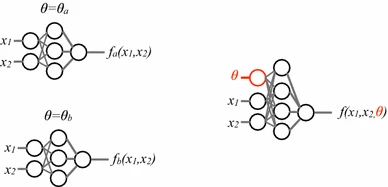
\includegraphics[width=.6\textwidth,keepaspectratio=true]{chapters/chapter6_HPlus/images/PNN_Diagram.png}
			\end{center}
			\caption{\textit{Left}, individual networks with input variables $(x_{1},x_{2})$, each trained with examples with a single value of some parameter $\theta = \theta_{a}, \theta_{b}$. The individual networks are purely functions of the input variables. Performance for intermediate values of $\theta$ is not optimal nor does it necessarily vary smoothly between the networks. \textit{Right}, a single network trained with input variables $(x_{1},x_{2})$ as well as input parameter $\theta$; such a network is trained with examples at several values of the parameter $\theta$ \cite{PNN}.}
			\label{fig:PNN-diagram}
		\end{figure}	

			This analysis uses four PNNs, events with 1-prong $\tau$ and 3-prong $\tau$ are divided into separate datasets within both subchannels.

		\subsection{Training}\label{ssec:training}
			The training of the PNNs used in this dissertation are done with the Keras \cite{keras} library using the TensorFlow \cite{tensorflow2015-whitepaper} library as backend. In order to increase the significance of training statistics and protect from overtraining, the $k$-fold method is used. Overtraining occurs when a NN has been fine tuned to have a high accuracy with a specific dataset and does not generalize to other datasets. To protect against this, dropout is used \cite{dropout}. The $k$-fold method divides input training samples into $k$ equally populated subsets. The $k$-th subset is trained on the other $k-1$ subsets and evaluated on the $k$-th subset. Figure \ref{fig:k-fold-diagram} shows a pictorial representation of the $k$-fold method. $k=5$ is chosen in this analysis.

			\begin{figure}	
				\begin{center}
					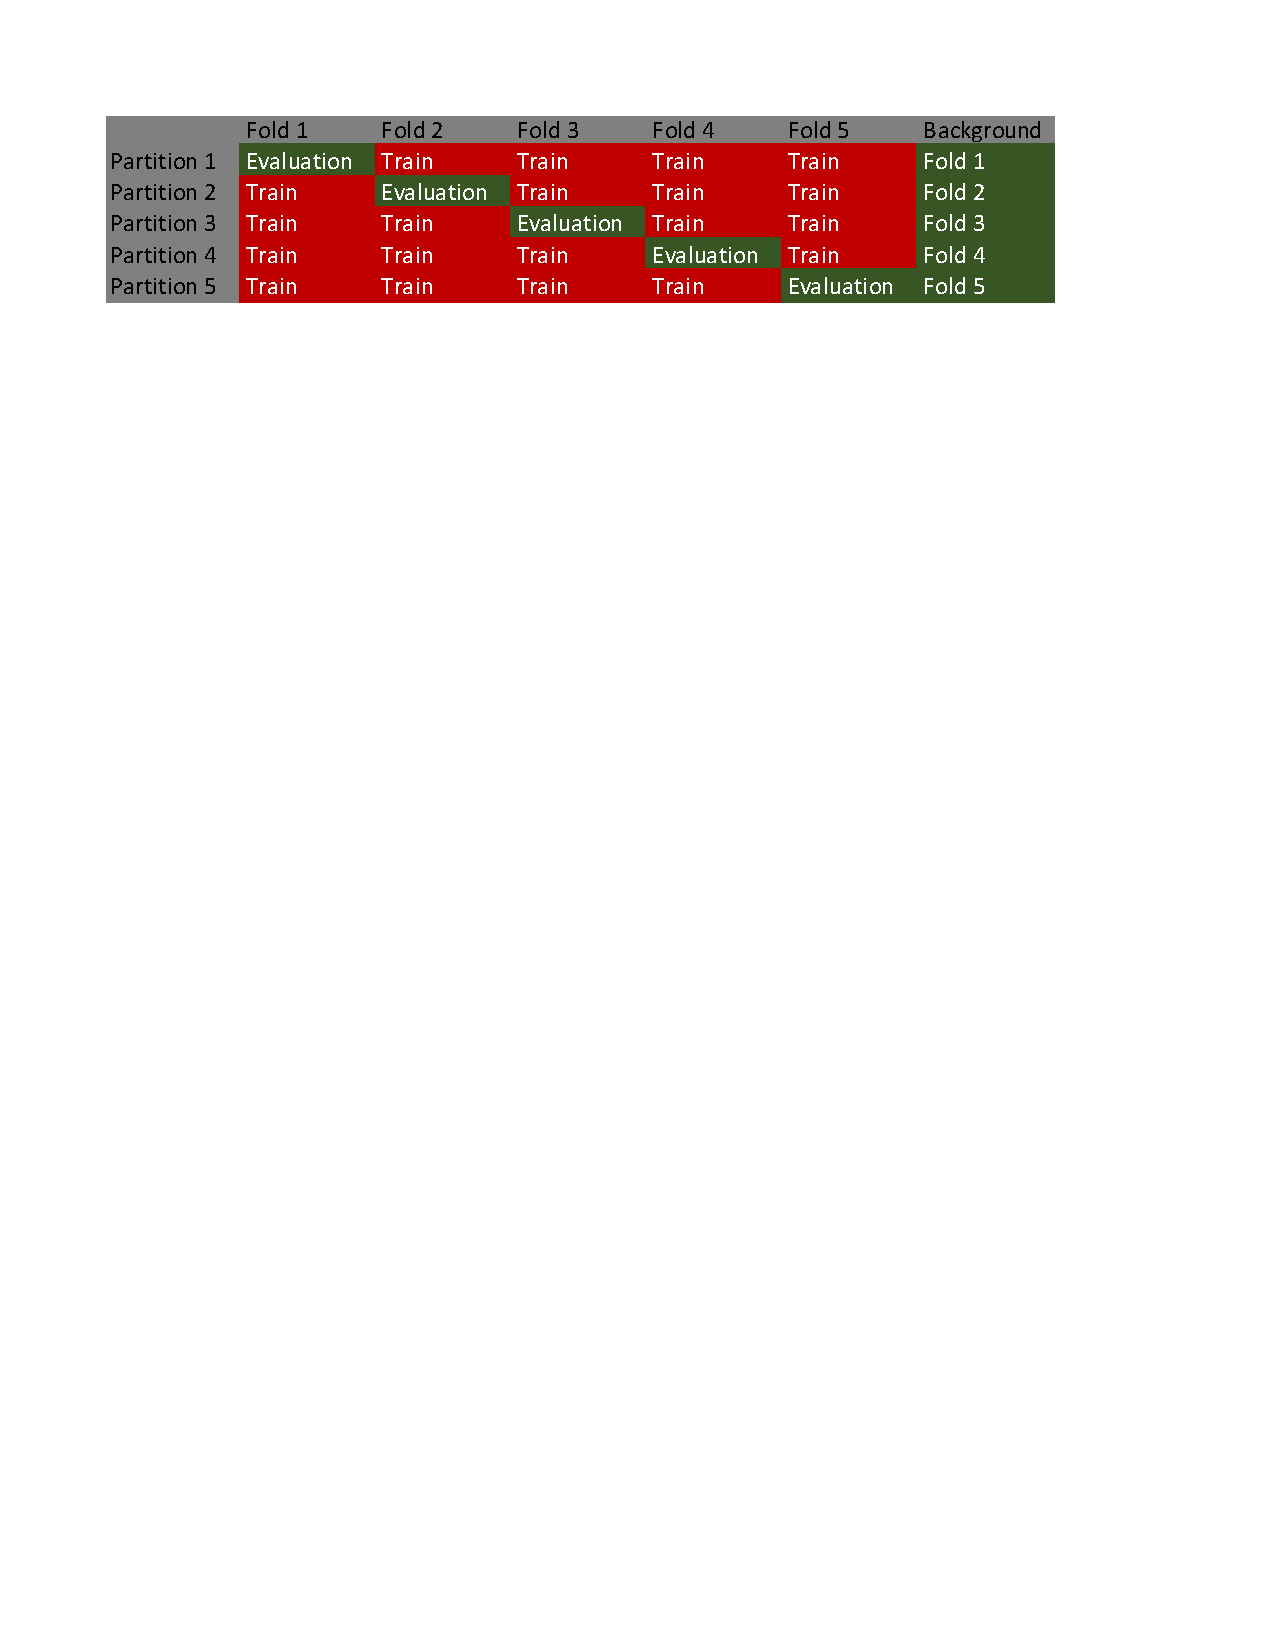
\includegraphics[width=.75\textwidth,keepaspectratio=true]{chapters/chapter6_HPlus/images/kFoldDiagram_noValid.pdf}
				\end{center}
				\caption{The k-fold method for $k=5$ \cite{Burghgrave:2018uwq}.}
				\label{fig:k-fold-diagram}
			\end{figure}	

			A single PNN training is performed on all \mHpm values at once, with the \mHpm value being taken as an input variable. For signal events, the \mHpm value from the MC generator is given; background events are replicated 32 times (the number of simulated \mHpm points is 32) and each \mHpm value is given for each set. To avoid biasing the training due to varying statistics at each \mHpm value, the background events are weighted by a factor of $w = N^{i}_{S}/N^{i}_{B}$ where $i$ corresponds to a given \mHpm value, $N^{i}_{S}$, and $N^{i}_{B}$ are the number of signal and background events respectively. When the PNN is evaluated, the \mHpm value is chosen and the output is used as the discriminant at that \mHpm.

		\subsection{Input Variables Selection}\label{ssec:input-variables}
			The choice of input variables to the PNNs is critical to the performance of the analysis. Several sets of variables were compared using expected limits as the figure of merit. All studies were performed in the \taulep signal region, as this region proves the most difficult challenge to separate signal-like events from background-like events. So called low level variables, consisting of the four vector components of the main physics objects in each event, were compared against high level variables; high level meaning they are calculated quantities from the low level variables. Tables of the low level and high level variables are shown in Table \ref{tab:taulep-input-variables-high-v-low}. 

			The variable $\mHpm^{Truth}$ corresponds to the \mHpm value the training and evaluation is performed at. In both cases, the variable $\Upsilon$ is used. $\Upsilon$ is a measure of the \tauhad polarization, computed by taking the asymmetry of energies carried by the charged and neutron pions from the 1-prong $\tau$ decay measured in the laboratory frame. $\Upsilon$ is defined as
			\begin{equation}\label{eqn:upsilon}
			\Upsilon = \frac{ E^{\pi^{\pm}}_{T} - E^{\pi^{0}}_{T}}{E^{\tau}_{T}} \approx 2 \frac{\pt^{\tau-\mathrm{track}}}{\pt^{\tau}} -1
			\end{equation}
			where $\pt^{\tau-\mathrm{track}}$ is the transverse momentum of the track associated with the 1-prong \tauhad candidate. As such, $\Upsilon$ is only defined for 1-prong \tauhad candidates. As demonstrated in the previous analysis, $\Upsilon$ provides a large contribution to signal-backgrounds separation at charged Higgs masses below 400 GeV \cite{hpm-previous}.

			% \begin{table}[!ht]
			% 	\begin{center}
			% 	\caption{List of high level kinematic variables used as input to the PNN in the \taulep subchannel. $\Delta \phi_{X,\,\text{miss}}$ denotes the difference in azimuthal angle between a reconstructed object $X$ ($X = \tauhad,\,\bjet,\,\ell$) and the direction of the missing transverse momentum.}
			% 	\begin{tabular}{| l |}
			% 	\hline
			% 	\textbf{High Level Input Variables} \\
			% 	\hline \hline
			% 	$\Etm$  \\
			% 	$\pt^{\tau}$  \\
			% 	$\pt^{\bjet}$  \\
			% 	$\pt^{\ell}$  \\
			% 	$\Delta \phi_{\tauhad,\,\text{miss}}$  \\
			% 	$\Delta \phi_{\bjet,\,\text{miss}}$  \\
			% 	$\Delta \phi_{\ell,\,\text{miss}}$  \\
			% 	$\Delta R_{\tauhad,\,\ell}$ \\
			% 	$\Delta R_{\bjet,\,\ell}$ \\
			% 	$\Delta R_{\bjet,\,\tauhad}$ \\
			% 	$\Delta \phi_{\tauhad, \text{miss}} / \Delta \phi_{\text{jet}, \text{miss}}$  \\
			% 	$\Upsilon$ \\
			% 	$\mHpm^{Truth}$ \\ \hline
			% 	\end{tabular}
			% 	\label{tab:pnn-high-level-input-variables}
			% 	\end{center}
			% \end{table}

		 %  \begin{table}[!ht]
		 %  	\begin{center}
		 %  	\caption{ List of low level kinematic variables used as input to the PNN in the \taulep subchannel.
		 %  	}
		  %     \begin{tabular}{| c | c | c | c |}
		  %       \multicolumn{4}{c}{\textbf{Low Level Input Variables}} \\ \hline \hline
		  %       $\pt^{\tau}$ & $\eta^{\tau}$ & $\phi^{\tau}$ & $E^{\tau}$ \\ \hline
		  %       $\pt^{\ell}$ & $\eta^{\ell}$ & $\phi^{\ell}$ & $E^{\ell}$ \\ \hline
		  %       $\pt^{\bjet}$ & $\eta^{\bjet}$ & $\phi^{\bjet}$ & $E^{\bjet}$ \\ \hline
		  %       $\pt^{jet}$ & $\eta^{jet}$ & $\phi^{jet}$ & $E^{jet}$ \\ \hline
		  %       \Etm & $\phi^{\Etm}$ & $\pt^{j_{1}}$ & $\Upsilon$  \\ \hline
		  %       $\mHpm^{Truth}$ & & & \\ \hline 
		  %       \hline
		  %       \end{tabular}
		  %       \label{tab:pnn-low-level-input-variables}
		  %       \end{center}
	   	%    \end{table}




      \begin{table}[!thp]
				\begin{subtable}[c]{0.25\textwidth}
					\centering
					\begin{tabular}{| c | c | c | c |}
		        \multicolumn{4}{c}{\textbf{Low Level Input Variables}} \\ \hline \hline
		        $\pt^{\tau}$ & $\eta^{\tau}$ & $\phi^{\tau}$ & $E^{\tau}$ \\ \hline
		        $\pt^{\ell}$ & $\eta^{\ell}$ & $\phi^{\ell}$ & $E^{\ell}$ \\ \hline
		        $\pt^{\bjet}$ & $\eta^{\bjet}$ & $\phi^{\bjet}$ & $E^{\bjet}$ \\ \hline
		        $\pt^{jet}$ & $\eta^{jet}$ & $\phi^{jet}$ & $E^{jet}$ \\ \hline
		        \Etm & $\phi^{\Etm}$ & $\pt^{j_{1}}$ & $\Upsilon$  \\ \hline
		        $\mHpm^{Truth}$ & & & \\ \hline 
	        \end{tabular}
	        \subcaption{Low level variables}
	      \end{subtable}

				\begin{subtable}[c]{0.25\textwidth}
					\centering
					\begin{tabular}{| l |}
						\hline
						\textbf{High Level Input Variables} \\
						\hline \hline
						$\Etm$  \\
						$\pt^{\tau}$  \\
						$\pt^{\bjet}$  \\
						$\pt^{\ell}$  \\
						$\Delta \phi_{\tau,\,\text{miss}}$  \\
						$\Delta \phi_{\bjet,\,\text{miss}}$  \\
						$\Delta \phi_{\ell,\,\text{miss}}$  \\
						$\Delta R_{\tau,\,\ell}$ \\
						$\Delta R_{\bjet,\,\ell}$ \\
						$\Delta R_{\bjet,\,\tau}$ \\
						$\Delta \phi_{\tau, \text{miss}} / \Delta \phi_{\text{jet}, \text{miss}}$  \\
						$\Upsilon$ \\
						$\mHpm^{Truth}$ \\ \hline
					\end{tabular}
					\subcaption{High level variables}
				\end{subtable}
				\caption{List of low level (a) and high level (b) kinematic variables used as input to the PNN in the \taulep subchannel. $\Delta \phi_{X,\,\text{miss}}$ denotes the difference in azimuthal angle between a reconstructed object $X$ ($X = \tau,\,\bjet,\,\ell$) and the direction of the missing transverse momentum.}
				\label{tab:taulep-input-variables-high-v-low}
			\end{table}

      An estimate of the impact of low level vs high level variables on the expected limits on $\sigma(\pp\to tb\Hpm)\times \mathrm{\cal{B}}(\Hpm \to \tau \nu)$ is shown in \ref{fig:variable-comparison-limits}. The set of low level variables was chosen as performance was similar in low \mHpm and greater in high \mHpm. A optimization of the number of layers in the PNN and several other parameters of the PNN is discussed in detail in Section \ref{ssec:hpo}.
			\begin{figure}	
				\begin{center}
					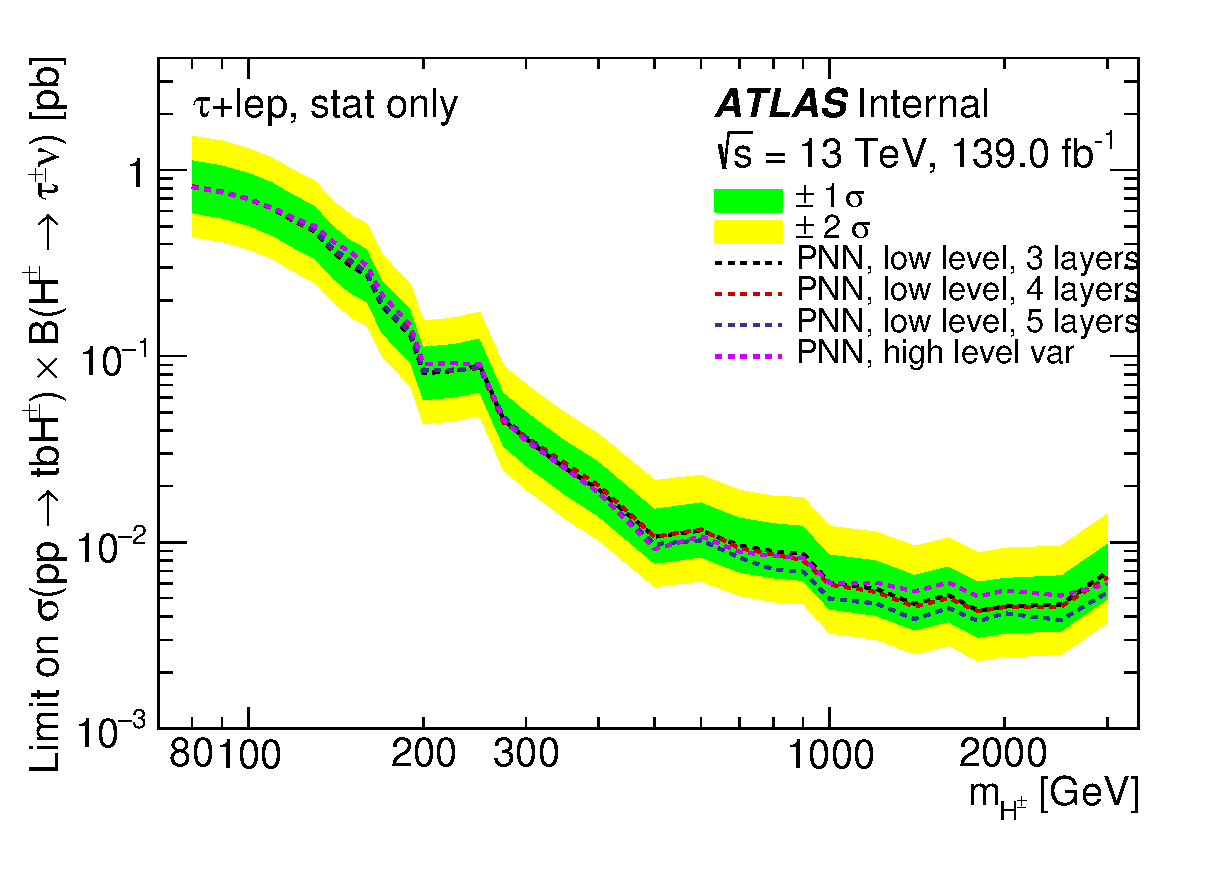
\includegraphics[width=.75\textwidth,keepaspectratio=true]{chapters/chapter6_HPlus/images/taulep_limits_PNN_low_lv_vs_high_lv.eps}
				\end{center}
				\caption{Expected limits comparing a set of high level variables and low level variables with various depths in the PNN architecture. X layers refers to the number of layers in the PNN. }
				\label{fig:variable-comparison-limits}
			\end{figure}	

		\subsection{Hyperparameter Optimization}\label{ssec:hpo}

				In order to optimize the PNN, a scan of hyperparameters and network architecture was done, referred to as hyperparameter optimization (HPO). A calculated area under the curve, (AUC), was used as the figure of merit. As in the normal training scheme, the $k$-fold method with $k=5$ was used to keep background modelling and classifier training statistically independent. To prevent overtraining, the early stopping method was used with $\Delta_{min}=0.00001$ and a patience of 10, with the best weights kept to calculate the AUC. To optimize for PNN performance in low \Hpm mass points, a separate average taking into account only \Hpm mass values between $80$ and $500$ GeV was used as the final figure of merit. In an effort to keep the computational needs low, several small grids of hyperparameters and architecture structures were scanned. Tables \ref{Tab:taulepHPOLoss} - \ref{Tab:taulepHPOWidthDepth} show the hyperparameter grids that were searched. Here, width refers to the number of neurons per layer and depth is the number of layers. The final hyperparameter from each grid search is highlighted in red. The results of the final grid search can be seen in Tables \ref{tab:pnn_hpo_aucs} and \ref{tab:pnn_hpo_aucs_short}; the quoted errors are taken from the different $k$-folds. The AUC values for each \mHpm point for the final chosen model are shown in Figure \ref{fig:final-auc}. 


			\begin{table}[!htb]
			  \begin{center}
					\resizebox{.65\textwidth}{!}{
			    \begin{tabular}{c | c | c | c}
			    Parameter  \\
			    \hline
			    activation function & softsign & relu & LeakyReLU \\ \hline
			    loss function & \fcolorbox{red}{white}{binary crossentropy} & mean squared error & mean absolute error \\ \hline
			    width & 32 & & \\ \hline
			    depth & 10 & & \\ \hline
			    batch size & 1025 &  & \\ \hline
			    \end{tabular}}
			    \caption{
			      First grid, scanning over activation function and loss function. Binary crossentropy was the chosen loss function, highlighted in red.
			    }
			    \label{Tab:taulepHPOLoss}
			  \end{center}
			\end{table}


			\begin{table}[!htb]
			  \begin{center}
					\resizebox{.55\textwidth}{!}{
			    \begin{tabular}{c | c | c | c}
			    Parameter  \\
			    \hline
			    width & 8 & 16 & 32 \\ \hline
			    depth & 3 & 5 & 10 \\ \hline
			    dropout & \fcolorbox{red}{white}{0.1} & 0.3 & \\ \hline
			    activation function & softsign & & \\ \hline
			    loss function & binary crossentropy & & \\ \hline 
			    batch size & 1024 &  & \\ \hline
			    \end{tabular}}
			    \caption{\label{Tab:taulepHPODropout}
			      Second grid, scanning over width, depth, and dropout value. $0.1$ was chosen for the dropout value, highlighted in red.
			    }
			  \end{center}
			\end{table}

			\begin{table}[!htb]
			  \begin{center}
				\resizebox{.55\textwidth}{!}{
			    \begin{tabular}{c | c | c | c}
			    Parameter  \\
			    \hline
			    width & 32 & 64 & 128 \\ \hline
			    depth & 2 & 3 & 4 \\ \hline
			    activation function & softsign & relu & \fcolorbox{red}{white}{LeakyReLU} \\ \hline
			    dropout & 0.1 & & \\ \hline
			    batch size & 1024 &  & \\ \hline
			    loss function & binary crossentropy  & & \\ \hline
			    \end{tabular}}
			    \caption{\label{Tab:taulepHPOActivation}
			      Third grid, scanning over activation function. LeakyReLU was chosen, highlighted in red.
			    }
			    
			  \end{center}
			\end{table}


			\begin{table}[!htb]
			  \begin{center}
				\resizebox{.55\textwidth}{!}{
			  \begin{tabular}{c | c | c | c | c}
			  Parameter  \\ 
			  \hline
			  width & 32 & 64 & 128 & \\ \hline
			  depth & 2 & 3 & 4 &  \\ \hline
			  $\alpha$ & 0.01 & \fcolorbox{red}{white}{0.05} & 0.001 & 0.005 \\ \hline
			  batch size & 1024 & & & \\ \hline
			  dropout & 0.1 & & & \\ \hline
			  activation function & LeakyReLU &  &  &  \\ \hline
			  loss function & binary crossentropy & & &  \\ \hline
			  \end{tabular}}
			    \caption{\label{Tab:taulepHPOAlpha}
			      Fourth grid, scanning over LeakyReLU $\alpha$ value. $\alpha=0.05$ was chosen, highlighted in red.
			    }
			    
			  \end{center}
			\end{table}

			\begin{table}[!htb]
			  \begin{center}
				\resizebox{.55\textwidth}{!}{
			  \begin{tabular}{c | c | c | c | c}
			  Parameter  \\ 
			  \hline
			  width & 32 & 64 & \fcolorbox{red}{white}{128} & 256 \\
			  depth & 2 & \fcolorbox{red}{white}{3} & 4 & 5 \\
			  batch size & 1024 &  & & \\ \hline
			  dropout & 0.1 &  &  &  \\ \hline
			  activation function & LeakyReLU &  &  &  \\ \hline
			  batch size & 1024 & & & \\ \hline
			  $\alpha$ & 0.05 &  &  &  \\ \hline
			  loss function & binary crossentropy & & &  \\ \hline
			  \end{tabular}}
			    \caption{\label{Tab:taulepHPOWidthDepth}
			      Fourth grid, scanning over network width and depth. $width=128$ and $depth=3$ was chosen, highlighted in red.
			    }
			    
			  \end{center}
			\end{table}

			\begin{table}
				\begin{center}
				\small
				\resizebox{\textwidth}{!}{
				\begin{tabular}{llrrrrrrrrrrrr}
				\toprule
				width & depth &         80 &       150 &       250 &       500 &       Avg &   LowMassAvg \\
				\midrule
				128 &     3 &  0.666137 $\pm$  0.000000 &  0.814508 $\pm$  0.000000 &  0.903123 $\pm$  0.000000 &  0.963256 $\pm$  0.000000 &  0.887638 $\pm$ 0.000000 &  0.826145 $\pm$ 0.096754 \\
				 128 &     5 &  0.649154 $\pm$  0.000000 &  0.804344 $\pm$  0.000000 &  0.907763 $\pm$  0.000000 &  0.962846 $\pm$  0.000000 &  0.886060 $\pm$ 0.000000 &  0.823542 $\pm$ 0.100037 \\
				 128 &     4 &  0.659330 $\pm$  0.000000 &  0.811707 $\pm$  0.000000 &  0.901186 $\pm$  0.000000 &  0.963811 $\pm$  0.000000 &  0.885833 $\pm$ 0.000000 &  0.823208 $\pm$ 0.099379 \\
				 128 &     2 &  0.644392 $\pm$  0.000000 &  0.807016 $\pm$  0.000000 &  0.907517 $\pm$  0.000000 &  0.963076 $\pm$  0.000000 &  0.885685 $\pm$ 0.000000 &  0.823139 $\pm$ 0.100649 \\
				  64 &     4 &  0.657593 $\pm$  0.005023 &  0.807977 $\pm$  0.001327 &  0.905193 $\pm$  0.004490 &  0.965553 $\pm$  0.001622 &  0.885708 $\pm$ 0.000177 &  0.823001 $\pm$ 0.099420 \\
				  64 &     2 &  0.652767 $\pm$  0.006639 &  0.805184 $\pm$  0.002345 &  0.905695 $\pm$  0.003172 &  0.965077 $\pm$  0.000726 &  0.885537 $\pm$ 0.000443 &  0.822775 $\pm$ 0.099628 \\
				  64 &     5 &  0.653787 $\pm$  0.005006 &  0.804417 $\pm$  0.001933 &  0.905833 $\pm$  0.003671 &  0.965293 $\pm$  0.001398 &  0.885338 $\pm$ 0.000545 &  0.822360 $\pm$ 0.099660 \\
				  64 &     3 &  0.652007 $\pm$  0.006721 &  0.805076 $\pm$  0.001760 &  0.904237 $\pm$  0.004398 &  0.964922 $\pm$  0.001898 &  0.885317 $\pm$ 0.001074 &  0.822335 $\pm$ 0.099360 \\
				 256 &     5 &  0.653576 $\pm$  0.000963 &  0.804396 $\pm$  0.003342 &  0.903638 $\pm$  0.004193 &  0.964415 $\pm$  0.002172 &  0.884405 $\pm$ 0.000175 &  0.821347 $\pm$ 0.100307 \\
				 256 &     4 &  0.643401 $\pm$  0.000000 &  0.801775 $\pm$  0.000000 &  0.901747 $\pm$  0.000000 &  0.961914 $\pm$  0.000000 &  0.882293 $\pm$ 0.000000 &  0.818097 $\pm$ 0.101322 \\
				  32 &     3 &  0.636902 $\pm$  0.009356 &  0.794963 $\pm$  0.004126 &  0.897744 $\pm$  0.003173 &  0.963498 $\pm$  0.002178 &  0.879826 $\pm$ 0.001226 &  0.813868 $\pm$ 0.103095 \\
				  32 &     4 &  0.638362 $\pm$  0.003653 &  0.793516 $\pm$  0.003269 &  0.898635 $\pm$  0.003664 &  0.963582 $\pm$  0.001635 &  0.879864 $\pm$ 0.000928 &  0.813853 $\pm$ 0.103071 \\
				  32 &     2 &  0.639871 $\pm$  0.005791 &  0.792428 $\pm$  0.002366 &  0.898305 $\pm$  0.003283 &  0.962854 $\pm$  0.002313 &  0.879603 $\pm$ 0.000405 &  0.813528 $\pm$ 0.102342 \\
				  32 &     5 &  0.634979 $\pm$  0.007666 &  0.793076 $\pm$  0.005599 &  0.898086 $\pm$  0.002238 &  0.962539 $\pm$  0.000514 &  0.879239 $\pm$ 0.001076 &  0.812845 $\pm$ 0.103520 \\
				 256 &     2 &  0.632035 $\pm$  0.004384 &  0.797129 $\pm$  0.000014 &  0.893944 $\pm$  0.003417 &  0.958731 $\pm$  0.001777 &  0.878091 $\pm$ 0.000165 &  0.811994 $\pm$ 0.102326 \\
				\bottomrule
				\end{tabular}}
				\caption{\label{tab:pnn_hpo_aucs}
				AUCs of final HPO grid
				  }
				  \end{center}
			\end{table}
			% \clearpage

			\begin{table}
				\begin{center}
				\small
				\resizebox{.5\textwidth}{!}{
				\begin{tabular}{llrrrrrrrrrrrr}
				\toprule
				width & depth &  Avg &   LowMassAvg \\
				\midrule
				128  &     3 &   0.887638 $\pm$ 0.000000 &  0.826145 $\pm$ 0.096754 \\
				 128 &     5 &   0.886060 $\pm$ 0.000000 &  0.823542 $\pm$ 0.100037 \\
				 128 &     4 &   0.885833 $\pm$ 0.000000 &  0.823208 $\pm$ 0.099379 \\
				 128 &     2 &   0.885685 $\pm$ 0.000000 &  0.823139 $\pm$ 0.100649 \\
				  64 &     4 &   0.885708 $\pm$ 0.000177 &  0.823001 $\pm$ 0.099420 \\
				  64 &     2 &   0.885537 $\pm$ 0.000443 &  0.822775 $\pm$ 0.099628 \\
				  64 &     5 &   0.885338 $\pm$ 0.000545 &  0.822360 $\pm$ 0.099660 \\
				  64 &     3 &   0.885317 $\pm$ 0.001074 &  0.822335 $\pm$ 0.099360 \\
				 256 &     5 &   0.884405 $\pm$ 0.000175 &  0.821347 $\pm$ 0.100307 \\
				 256 &     4 &   0.882293 $\pm$ 0.000000 &  0.818097 $\pm$ 0.101322 \\
				  32 &     3 &   0.879826 $\pm$ 0.001226 &  0.813868 $\pm$ 0.103095 \\
				  32 &     4 &   0.879864 $\pm$ 0.000928 &  0.813853 $\pm$ 0.103071 \\
				  32 &     2 &   0.879603 $\pm$ 0.000405 &  0.813528 $\pm$ 0.102342 \\
				  32 &     5 &   0.879239 $\pm$ 0.001076 &  0.812845 $\pm$ 0.103520 \\
				 256 &     2 &   0.878091 $\pm$ 0.000165 &  0.811994 $\pm$ 0.102326 \\
				\bottomrule
				\end{tabular}}
				\caption{\label{tab:pnn_hpo_aucs_short}
				Average AUCs of final HPO grid
				  }
			  \end{center}
			\end{table}


			\clearpage
			\begin{figure}
			  \centering
			  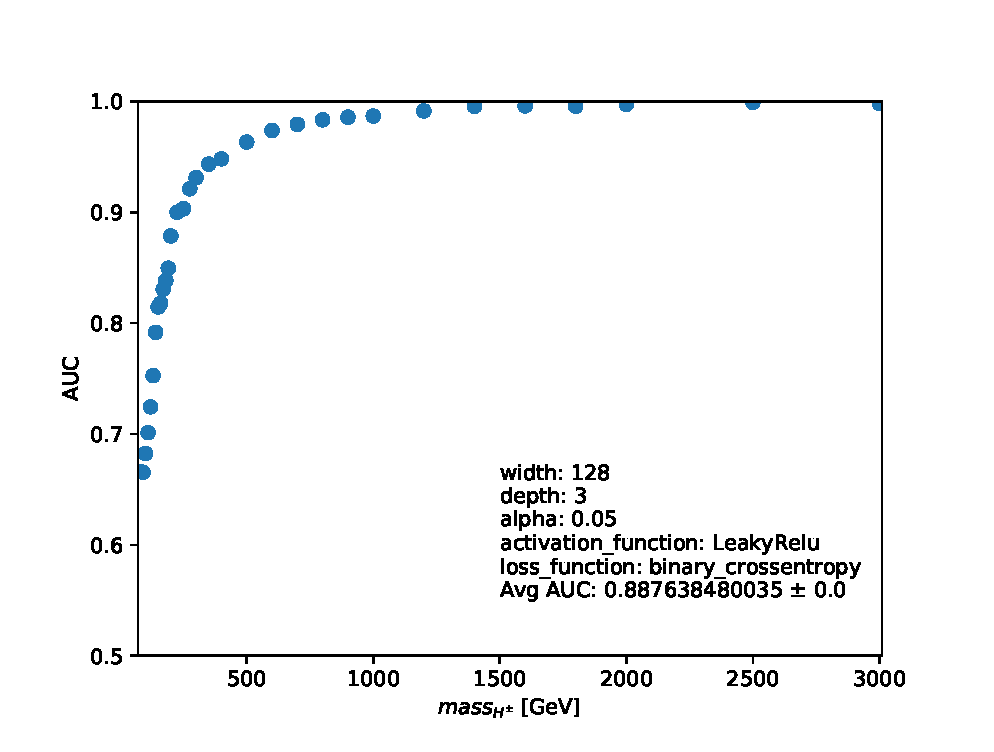
\includegraphics[width=\textwidth,keepaspectratio=true]{chapters/chapter6_Hplus/images/AUC_Plots/model_GB_1024_channel_taulep_mass_80to3000_ntracks_1_nfolds_5_fold_4_nvars_19_batch_size_1024_epochs_1000_dense_layer_size_128_activation_function_LeakyRelu_depth_3_loss_binary_crossentropy_dropout_0.1_alpha_0.05.eps}\\
			  \caption{Final model AUC for each mass point. Individual points correspond to the AUC average over 5 kfolds. }
			  \label{fig:final-auc}
			\end{figure}

			The final model was chosen to have 128 neurons per layer with 3 layers, with the binary crossentropy chosen as the loss function, a dropout of 0.1, LeakyReLU as the activation function with $\alpha=0.05$. The LeakyReLU activation function is depicted in Figure \ref{fig:leaky-relu}, where the $\alpha$ value is the slope of the negative portion. Allowing negative weight values prevents neurons from becoming deactivated prematurely.

			\begin{figure}
				\centering
				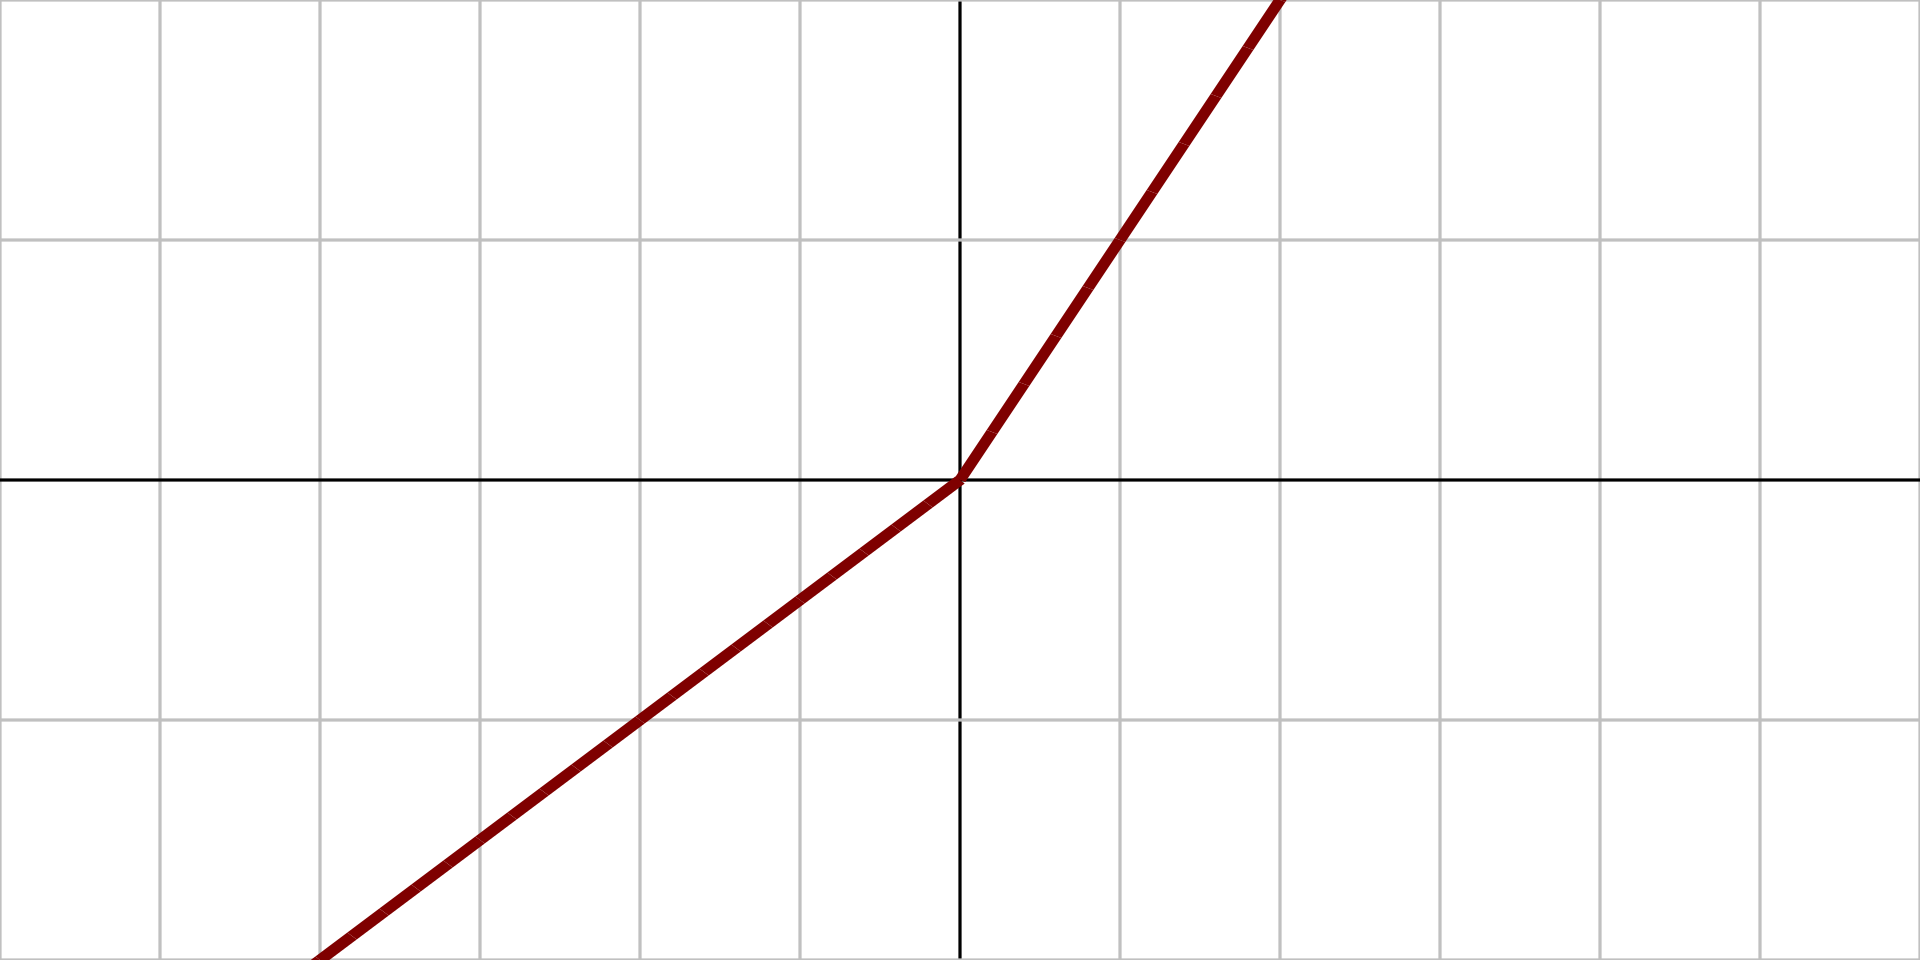
\includegraphics[width=.4\textwidth,keepaspectratio=true]{chapters/chapter6_HPlus/images/Activation_prelu.svg.png}
				\caption{LeakyReLU activation function. The associated hyperparameter $\alpha$ is the slope of the negative portion of the function.}
				\label{fig:leaky-relu}
			\end{figure}

	\section{Systematic Uncertainties}\label{sec:systs}
		Systematic uncertainties have a variety of sources and are discussed in detail here. Detector-related systematic uncertainties from the reconstruction and identification of leptons and \tauhad objects, simulation of the electron and muon triggers, reconstruction of \Etm, and energy/momentum scale and resolution of all physics objects are studied by varying selection cuts by $\pm 1$ standard deviation. The difference in event yields is then taken as a systematic error and summed in quadrature with all other sources of error to give the final quoted errors. Systematic uncertainties arising from the data-driven fake factor method are shown in Table \ref{tab:FF-syst-uncert}.

		\begin{table}[!htb]
		  \begin{center}
				\resizebox{\textwidth}{!}{
		    \begin{tabular}{l|c|c||c|c||}
		      &  \multicolumn{2}{c||}{\taujets}  & \multicolumn{2}{c||}{\taulep} \\
		      \hline
		      Source of uncertainty & Effect on yield & Shape & Effect on yield & Shape \\
		      \hline\hline
		      Fake factors: statistical uncertainties & 3.9$\%$ & \textcolor{red}{\checkmark} & 3.2$\%$ & \textcolor{red}{\checkmark}\\\hline
		      Fake factors: True $\tauhad$ in the anti-$\tauhad$ CR & \begin{tabular}{c}+3.4\% \\-3.2\%\end{tabular} & \textcolor{red}{\checkmark} & \begin{tabular}{c}+4\% \\-4.3\%\end{tabular} & \textcolor{red}{\checkmark}\\\hline
		      Fake factors: tau RNN Identification SF & 2.7$\%$ & \textcolor{red}{\checkmark} & 2.7$\%$ & \textcolor{red}{\checkmark}\\\hline
		      Fake factors: $\alpha_\text{MJ}$ uncertainty & 3.6\% & \textcolor{red}{\checkmark} & 1.9\% & \textcolor{red}{\checkmark}\\\hline
		      Fake factors: Smirnov transform & 0$\%$ & \textcolor{red}{\checkmark} & 0$\%$ & \textcolor{red}{\checkmark}\\\hline          
		      Fake factors: heavy flavor jet fraction & \textcolor{red}{5$\%$} & \textcolor{red}{\checkmark} & \textcolor{red}{5$\%$} & \textcolor{red}{\checkmark}\\
		    \end{tabular}}
		  \end{center}
		  \caption{\label{tab:FF-syst-uncert}
		    Effect on the shape variation and the yields of systematic uncertainties associated with the data-driven fake
		    factor method, used to estimate the $j \to \tau$ background in the
		   \taujets and \taulep channel.
		    }
		\end{table}

		Theoretical uncertainties for signal and \ttbar background were considered in the last publication; at the time of writing this dissertation the simulations are being produced and therefore are not included. 

		\textcolor{red}{Systematic \% difference wrt nominal is being finalized. Add in when done.}

	\section{Results}\label{sec:results}
		The expected event yields for backgrounds and signal\footnote{At the time of writing, the analysis is still blinded so Data is not included.} are summarized in Table \ref{tab:event_yields_SR_taujets} (\taujets) and Table \ref{tab:event_yields_SR_taulep} (\taulep).

		\begin{table}
			\begin{center}
			\caption{\label{tab:event_yields_SR_taujets} Expected event yields for the backgrounds and a hypothetical
			\Hpm signal after applying all \taujets selection criteria, and comparison with \LUMI of data. All yields
			are evaluated prior to using the multivariate discriminant and applying the statistical fitting procedure.
			The values shown for the signal assume a charged Higgs boson mass of 170 GeV and 1000 GeV, 
			with a cross-section times branching fraction $\sigma(\pp \to tb\Hpm) \times \mathrm{\cal{B}}(\Hpm \to \tau\nu)$ 
			corresponding to $\tanb=40$ in the hMSSM benchmark scenario. 
			Statistical 
			%and  
			uncertainties are quoted.
			%, respectively.
			\textcolor{red}{Systematic uncertainties to be added.}}

			\resizebox{0.75\textwidth}{!}{
			\begin{tabular}{l|l}
			Sample & Event yields $\tauhad$+jets          \\
			\hline
			True $\tau_{\text{had}}$  & \\
			\hspace*{5mm}\ttbar & $\phantom{}18369.33\phantom{.0}\pm\phantom{0}48.16\phantom{.0}\pm\phantom{0}XXX\phantom{.0}$    \\
			\hspace*{5mm}Single-top-quark  & $\phantom{0}2276.08\phantom{.0}\pm\phantom{0}16.69\phantom{.0}\pm\phantom{0}XXX\phantom{.0}$ \\
			\hspace*{5mm}$W \to \tau\nu$  & $\phantom{0}1972.76\phantom{.0}\pm\phantom{0}23.54\phantom{.0}\pm\phantom{0}XXX\phantom{.0}$  \\
			\hspace*{5mm}$Z \to \tau\tau$  & $\phantom{00}241.05\phantom{.0}\pm\phantom{00}5.47\phantom{.0}\pm\phantom{0}XXX\phantom{.0}$   \\
			\hspace*{5mm}Diboson ($WW, WZ, ZZ$) & $\phantom{00}133.30\phantom{.0}\pm\phantom{00}4.67\phantom{.0}\pm\phantom{0}XXX\phantom{0}$  \\
			Misidentified $e,\,\mu \to \tauhad$   & $\phantom{00}327.51\phantom{.0}\pm\phantom{00}6.82\phantom{.0}\pm\phantom{0}XXX\phantom{.0}$  \\
			Misidentified $\mbox{jet} \to \tauhad$ & $\phantom{0}2490.58\phantom{.0}\pm\phantom{0}17.35\phantom{.0}\pm \phantom{0}XXX\phantom{.0}$ \\
			\hline
			All backgrounds   & $25810.61\phantom{.0}\pm\phantom{0}59.60\phantom{.0}\pm\phantom{0} XXX\phantom{.0}$  \\
			\hline
			\Hpm $\phantom{0}$(170 GeV), hMSSM $\tanb=40$ & $\phantom{0}4330.22\phantom{.0}\pm\phantom{0}36.75\phantom{.0}\pm\phantom{0}XXX\phantom{.0}$  \\
			\Hpm (1000 GeV), hMSSM $\tanb=40$ & $\phantom{000}31.15\phantom{0.}\pm\phantom{00}0.14\phantom{0.}\pm\phantom{0}XXX$  \\
			\hline
			Data         &  XXX   \\
			\hline
			\end{tabular}}
			\end{center}
		\end{table}

		\begin{table}
			\begin{center}
			\caption{\label{tab:event_yields_SR_taulep} Expected event yields for the backgrounds and a hypothetical
			\Hpm signal after applying all \taulep selection criteria, and comparison with \LUMI of data. All yields
			are evaluated prior to using the multi-variate discriminant and applying the statistical fitting procedure. The
			values shown for the signal assume a charged Higgs boson mass of 170 GeV and 1000 GeV, 
			with a cross-section times branching fraction $\sigma(\pp \to tb\Hpm) \times \mathrm{\cal{B}}(\Hpm \to \tau\nu)$ 
			corresponding to $\tanb=40$ in the hMSSM benchmark scenario. 
			Statistical 
			%and  
			uncertainties are quoted.
			%, respectively.
			\textcolor{red}{Systematic uncertainties to be added.}}
			\resizebox{\textwidth}{!}{
			\begin{tabular}{l|l|l}
			Sample &   Event yields \tauel  & Event yields \taumu \\
			\hline
			True $\tau_{\text{had}}$  & \\
			\hspace*{5mm}$t\bar{t}$ & $43814.66\phantom{.0}\pm\phantom{0}76.84\phantom{.0}\pm\phantom{0} XXX$ & $44490.69\phantom{.0}\pm\phantom{0}75.96\phantom{.0}\pm\phantom{0} XXX$  \\
			\hspace*{5mm}Single-top-quark  & $\phantom{0}3260.70\phantom{.0}\pm\phantom{0}20.81\phantom{.0}\pm\phantom{0}XXX$ & $\phantom{0}3874.57\phantom{.0}\pm\phantom{0}22.06\phantom{.0}\pm\phantom{0}XXX$  \\
			\hspace*{5mm}$W \to \tau\nu$  & $\phantom{0000}2.41\phantom{.0}\pm\phantom{00}0.56\phantom{.0}\pm\phantom{0}XXX\phantom{.0}$ & $\phantom{0000}0.07\phantom{.0}\pm\phantom{00}0.12\phantom{.0}\pm\phantom{0}XXX\phantom{.0}$  \\
			\hspace*{5mm}$Z \to \tau\tau$  & $\phantom{00}913.61\phantom{.0}\pm\phantom{0}20.42\phantom{.0}\pm\phantom{0}XXX$  & $\phantom{00}845.89\phantom{.0}\pm\phantom{0}22.07\phantom{.0}\pm\phantom{0}XXX$ \\
			\hspace*{5mm}Diboson ($WW, WZ, ZZ$) &  $\phantom{000}73.21\phantom{.0}\pm\phantom{00}1.53\phantom{.0}\pm\phantom{0}XXX$ & $\phantom{000}81.32\phantom{.0}\pm\phantom{00}1.53\phantom{.0}\pm\phantom{0}XXX$ \\
			Misidentified $e,\,\mu \to \tauhad$   &   $\phantom{0}1096.64\phantom{.0}\pm\phantom{0}24.36\phantom{.0}\pm\phantom{0}XXX$ & $\phantom{0}1074.28\phantom{.0}\pm\phantom{0}15.90\phantom{.0}\pm\phantom{0}XXX$ \\
			Misidentified $\mbox{jet} \to \tauhad$ &   $\phantom{0}8773.81\phantom{.0}\pm\phantom{0}37.64\phantom{.0}\pm\phantom{0}XXX$ & $\phantom{0}8558.21\phantom{.0}\pm\phantom{0}37.23\phantom{.0}\pm\phantom{0}XXX$ \\
			\hline
			All backgrounds   &  $57935.04\phantom{.0}\pm\phantom{0} 93.63\phantom{.0}\pm\phantom{0} XXX$ & $58925.03\phantom{.0}\pm\phantom{0} 91.57\phantom{.0}\pm\phantom{0} XXX$ \\
			\hline
			\Hpm $\phantom{0}$(170 GeV), hMSSM $\tanb=40$ & $\phantom{0}2543.83\phantom{.0}\pm\phantom{0}28.12\phantom{.0}\pm\phantom{0}XXX$ & $\phantom{0}2877.49\phantom{.0}\pm\phantom{0}28.41\phantom{.0}\pm\phantom{0}XXX$ \\
			\Hpm (1000 GeV), hMSSM $\tanb=40$ &   $\phantom{0000}2.34\phantom{0.}\pm\phantom{00}0.03\phantom{0.}\pm\phantom{0}XXX$ & $\phantom{0000}2.46\phantom{0.}\pm\phantom{00}0.03\phantom{0.}\pm\phantom{0}XXX$ \\
			\hline
			Data         &     XXX &  XXX  \\
			\hline
			\end{tabular}}
			\end{center}
		\end{table}

		The test statistic $\tilde{q}_{\mu}$ \cite{test-statistic} is used to test the agreement of the data with the background-only and signal+background hypotheses. The test statistic is based on a profile likelihood ratio where the binned likelihood function $\cal{L}(\mu,\theta)$ is constructed as the product of Poisson probability terms over all bins and regions. The likelihood ratio is the ratio between the conditional maximum-likelihood estimator of the nuisance parameters, $\theta$, for a given signal hypothesis $\mu$ and the unconditional maximum-likelihood estimator for $\mu$ and the nuisance parameters. $\tilde{q}_{\mu}$ is defined as:
		\begin{equation}
		\tilde{q}_{\mu} = \left\{
		\begin{array}{ll}
		-2\ln\frac{{\cal L}(\mu, \hat{\hat{\theta}}(\mu))}{{\cal L}(0, \hat{\hat{\theta}}(0))}, & \hat{\mu} < 0 \\
		-2\ln\frac{{\cal L}(\mu, \hat{\hat{\theta}}(\mu))}{{\cal L}(\hat{\mu}, \hat{\theta})}, & 0 \leq \hat{\mu} \leq \mu \\
		0 & \hat{\mu} > \mu 
		\end{array}
		\right.
		\end{equation}

		The fit is performed on the PNN score distributions in the three signal regions, \taujets, \tauel, \taumu, and the dilepton-btag control region which is enriched in the dominant \ttbar background. Pre-fit PNN score distributions are shown in Figures \ref{fig:taujets_SR_PNNscores_body}, \ref{fig:taulepPNNscoreSR1_body}, and \ref{fig:taulepPNNscoreSR2_body}. At the time of writing this dissertation, the analysis is still blinded. Assuming the fit agrees with the background-only hypothesis expected limits of $\sigma(\pp \to tb\Hpm)\times \mathrm{\cal{B}}(\Hpm \to \tau \nu)$ are calculated. Exclusion limits are set at the 95\% confidence level (CL) using the $\mathrm{CL}_s$ procedure \cite{CL-setting}. The expected exclusion limits on $\sigma(\pp \to tb\Hpm)\times \mathrm{\cal{B}}(\Hpm \to \tau \nu)$ can be seen in Figure \ref{fig:expected-limits}.

		\begin{figure}
		  \centering
		\subfloat[\label{fig:taujets_SR_PNNscores_body_a}]{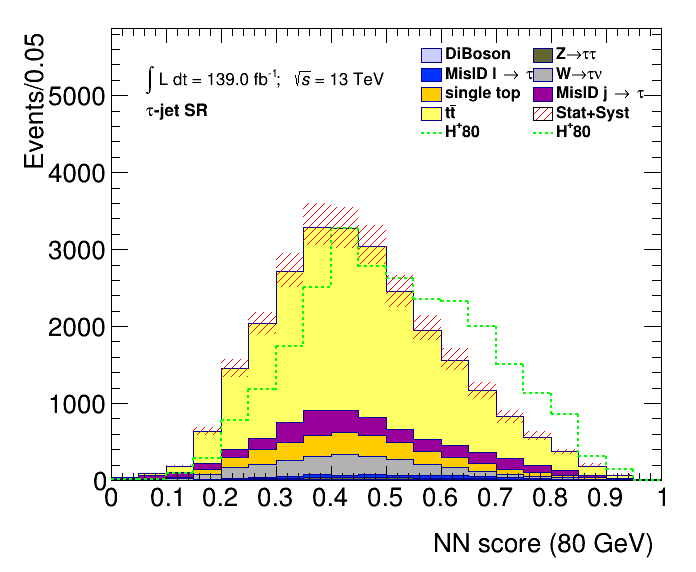
\includegraphics[width=0.45\linewidth]{chapters/chapter6_HPlus/images/taujets/clf_score_GB200_mass_80to80_SR_TAUJET.png}}
		\subfloat[\label{fig:taujets_SR_PNNscores_body_b}]{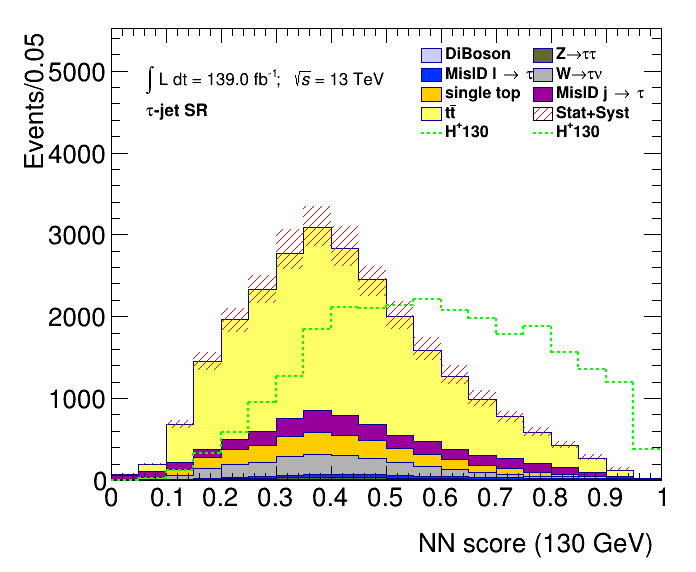
\includegraphics[width=0.45\linewidth]{chapters/chapter6_HPlus/images/taujets/clf_score_GB200_mass_130to130_SR_TAUJET.png}} \\
		\subfloat[\label{fig:taujets_SR_PNNscores_body_c}]{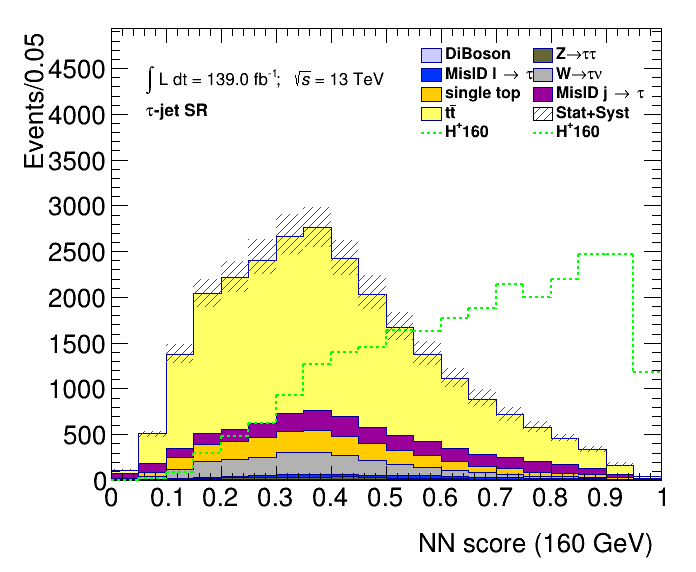
\includegraphics[width=0.45\linewidth]{chapters/chapter6_HPlus/images/taujets/clf_score_GB200_mass_160to160_SR_TAUJET.png}}
		\subfloat[\label{fig:taujets_SR_PNNscores_body_d}]{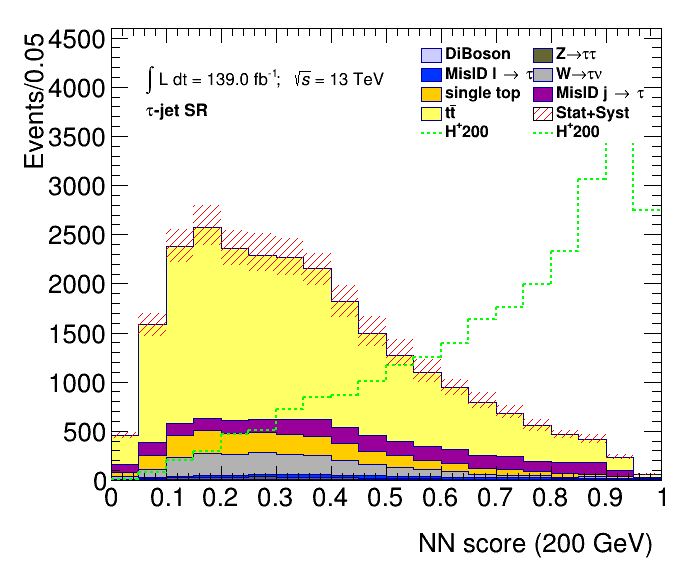
\includegraphics[width=0.45\linewidth]{chapters/chapter6_HPlus/images/taujets/clf_score_GB200_mass_200to200_SR_TAUJET.png}} \\
		\subfloat[\label{fig:taujets_SR_PNNscores_body_e}]{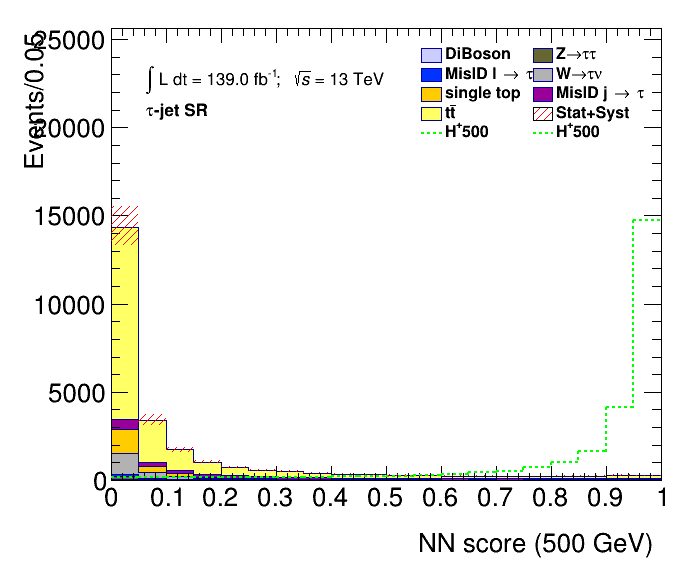
\includegraphics[width=0.45\linewidth]{chapters/chapter6_HPlus/images/taujets/clf_score_GB200_mass_500to500_SR_TAUJET.png}}
		\subfloat[\label{fig:taujets_SR_PNNscores_body_f}]{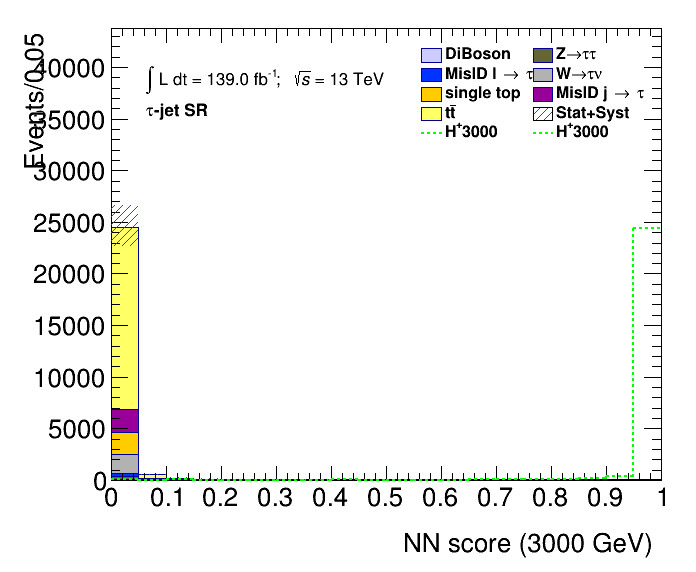
\includegraphics[width=0.45\linewidth]{chapters/chapter6_HPlus/images/taujets/clf_score_GB200_mass_3000to3000_SR_TAUJET.png}}
		  \caption{\label{fig:taujets_SR_PNNscores_body} PNN score distributions in the
		signal region of the \taujets channel, for the six charged Higgs boson mass parameters.
		The lower panel of each plot shows the ratio of data to the SM background prediction. The uncertainty bands include all statistical and systematic uncertainties. 
		The normalization of the signal (shown for illustration) corresponds to the integral of the background.}
		\end{figure}

		\begin{figure}
		\centering
		\subfloat[\label{fig:taulepPNNscoreSR1_body_a}]{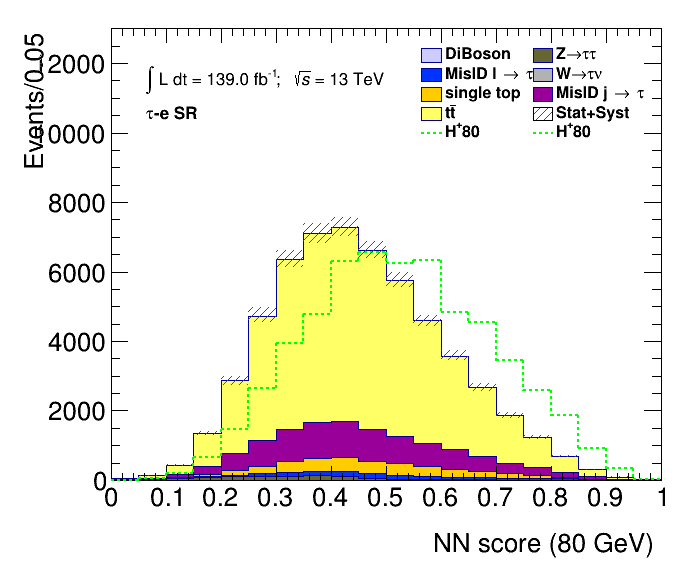
\includegraphics[width=0.45\linewidth]{chapters/chapter6_HPlus/images/taulep/clf_score_GB200_mass_80to80_SR_TAUEL.png}}
		\subfloat[\label{fig:taulepPNNscoreSR1_body_b}]{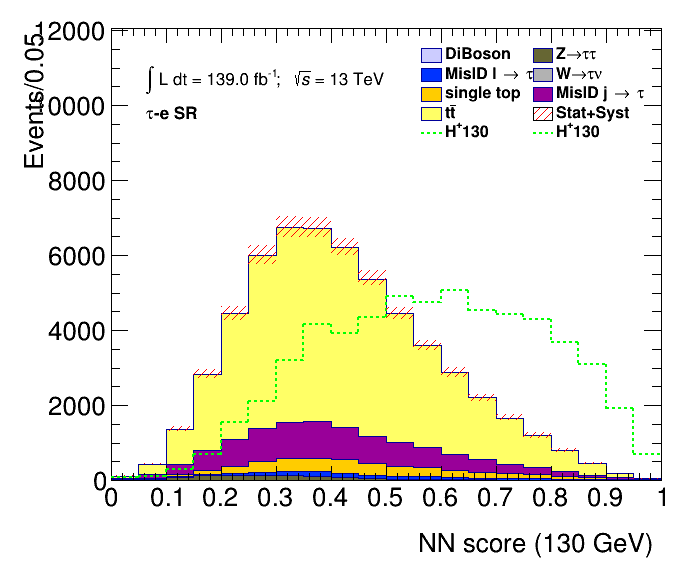
\includegraphics[width=0.45\linewidth]{chapters/chapter6_HPlus/images/taulep/clf_score_GB200_mass_130to130_SR_TAUEL.png}} \\
		\subfloat[\label{fig:taulepPNNscoreSR1_body_c}]{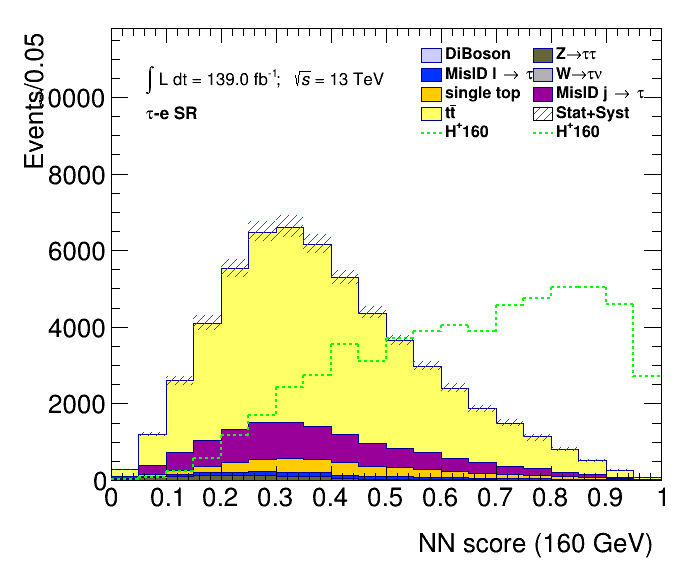
\includegraphics[width=0.45\linewidth]{chapters/chapter6_HPlus/images/taulep/clf_score_GB200_mass_160to160_SR_TAUEL.png}}
		\subfloat[\label{fig:taulepPNNscoreSR1_body_d}]{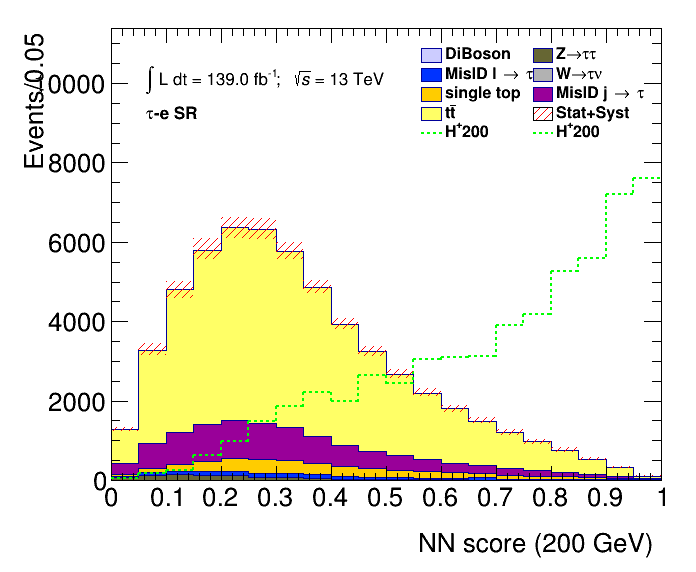
\includegraphics[width=0.45\linewidth]{chapters/chapter6_HPlus/images/taulep/clf_score_GB200_mass_200to200_SR_TAUEL.png}} \\
		\subfloat[\label{fig:taulepPNNscoreSR1_body_e}]{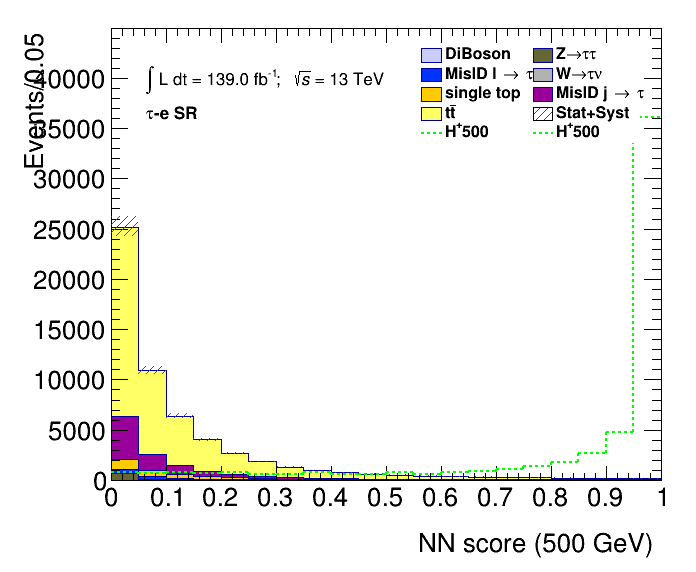
\includegraphics[width=0.45\linewidth]{chapters/chapter6_HPlus/images/taulep/clf_score_GB200_mass_500to500_SR_TAUEL.png}}
		\subfloat[\label{fig:taulepPNNscoreSR1_body_f}]{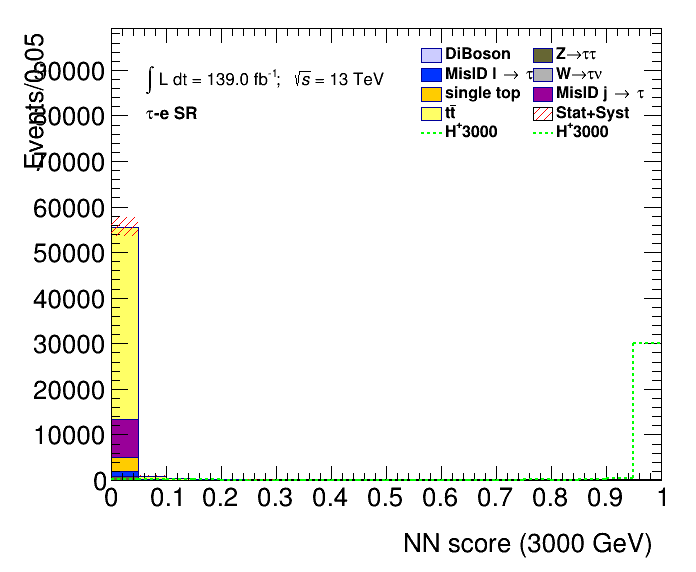
\includegraphics[width=0.45\linewidth]{chapters/chapter6_HPlus/images/taulep/clf_score_GB200_mass_3000to3000_SR_TAUEL.png}}
		\caption{\label{fig:taulepPNNscoreSR1_body} PNN score distributions in the
		signal region of the \tauel sub-channel, for the six charged Higgs boson mass parameters.
		The lower panel of each plot shows the ratio of data to the SM background prediction. The uncertainty bands include all statistical and systematic uncertainties.
		The normalization of the signal (shown for illustration) corresponds to the integral of the background.}
		\end{figure}

		\begin{figure}
		\centering
		\subfloat[\label{fig:taulepPNNscoreSR2_body_a}]{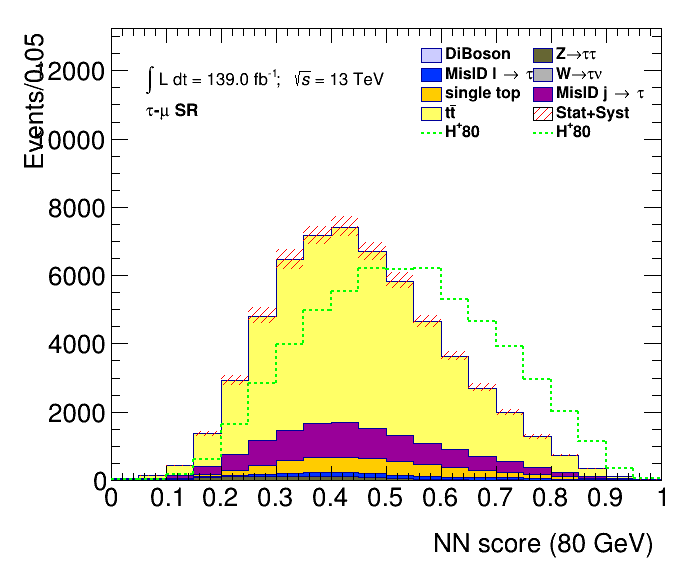
\includegraphics[width=0.45\linewidth]{chapters/chapter6_HPlus/images/taulep/clf_score_GB200_mass_80to80_SR_TAUMU.png}}
		\subfloat[\label{fig:taulepPNNscoreSR2_body_b}]{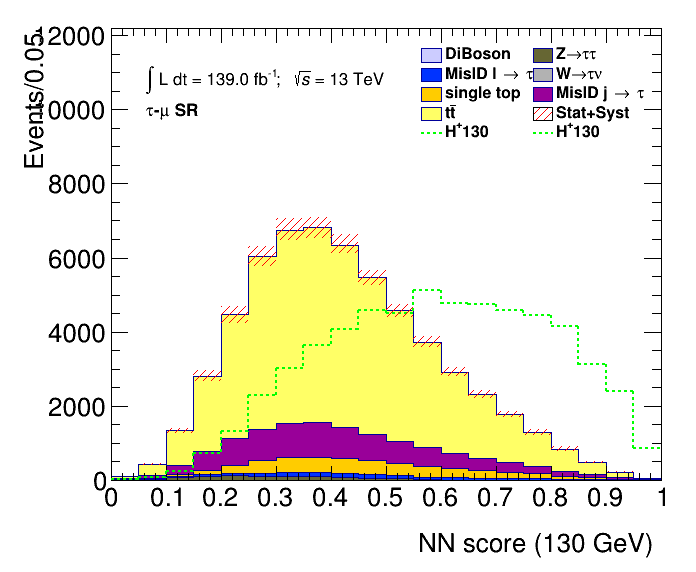
\includegraphics[width=0.45\linewidth]{chapters/chapter6_HPlus/images/taulep/clf_score_GB200_mass_130to130_SR_TAUMU.png}} \\
		\subfloat[\label{fig:taulepPNNscoreSR2_body_c}]{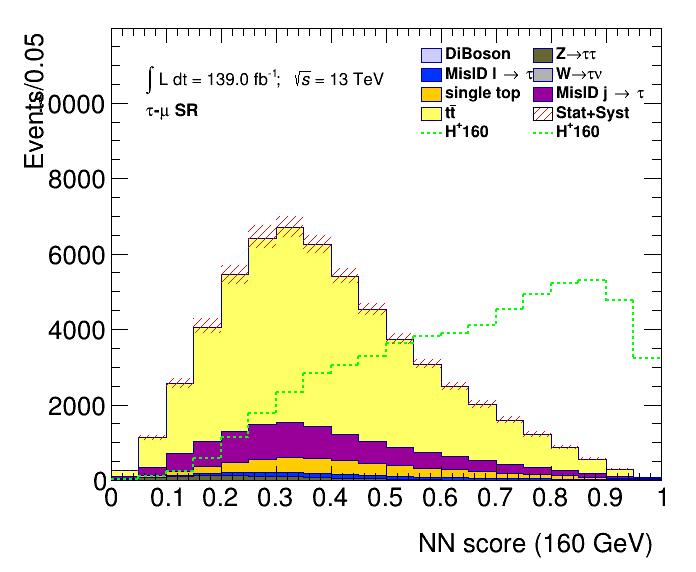
\includegraphics[width=0.45\linewidth]{chapters/chapter6_HPlus/images/taulep/clf_score_GB200_mass_160to160_SR_TAUMU.png}}
		\subfloat[\label{fig:taulepPNNscoreSR2_body_d}]{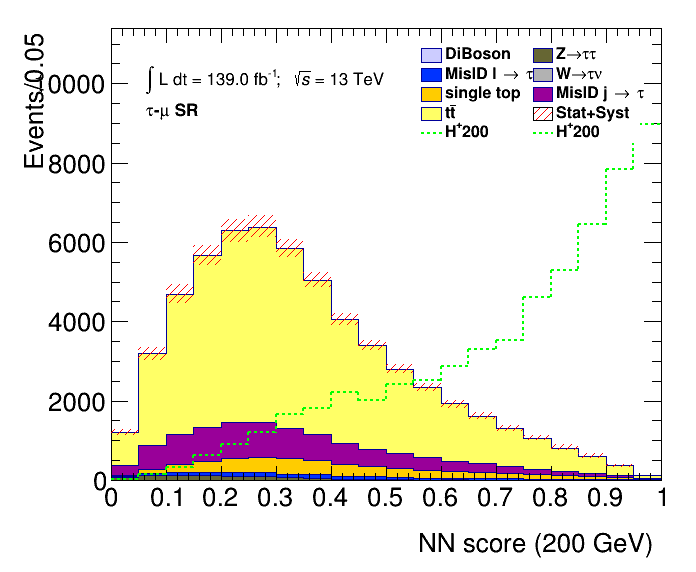
\includegraphics[width=0.45\linewidth]{chapters/chapter6_HPlus/images/taulep/clf_score_GB200_mass_200to200_SR_TAUMU.png}} \\
		\subfloat[\label{fig:taulepPNNscoreSR2_body_e}]{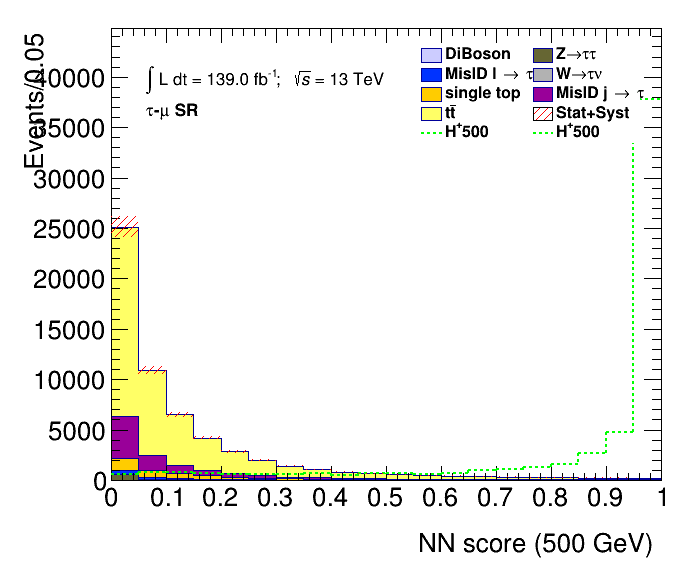
\includegraphics[width=0.45\linewidth]{chapters/chapter6_HPlus/images/taulep/clf_score_GB200_mass_500to500_SR_TAUMU.png}}
		\subfloat[\label{fig:taulepPNNscoreSR2_body_f}]{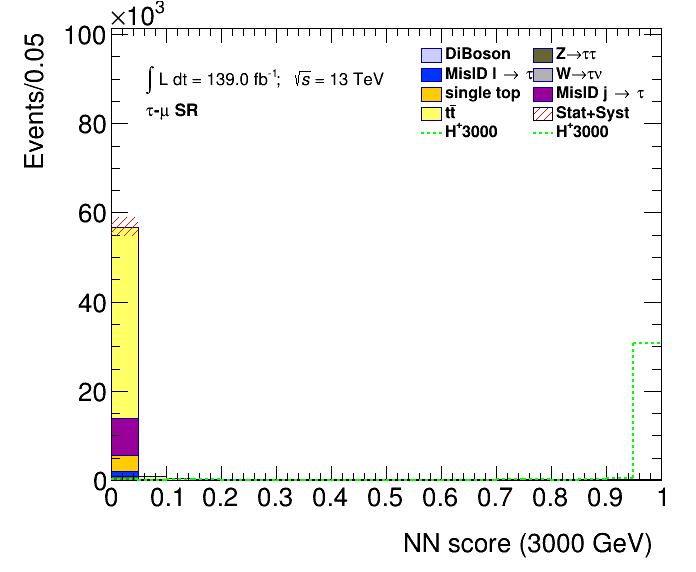
\includegraphics[width=0.45\linewidth]{chapters/chapter6_HPlus/images/taulep/clf_score_GB200_mass_3000to3000_SR_TAUMU.png}}
		\caption{\label{fig:taulepPNNscoreSR2_body} PNN score distributions in the
		signal region of the \taumu sub-channel, for the six charged Higgs boson mass parameters.
		The lower panel of each plot shows the ratio of data to the SM background prediction. The uncertainty bands include all statistical and systematic uncertainties.
		The normalization of the signal (shown for illustration) corresponds to the integral of the background.}
		\end{figure}

		\begin{figure}
		\centering
		\subfloat[\label{fig:expected-limits-a}]{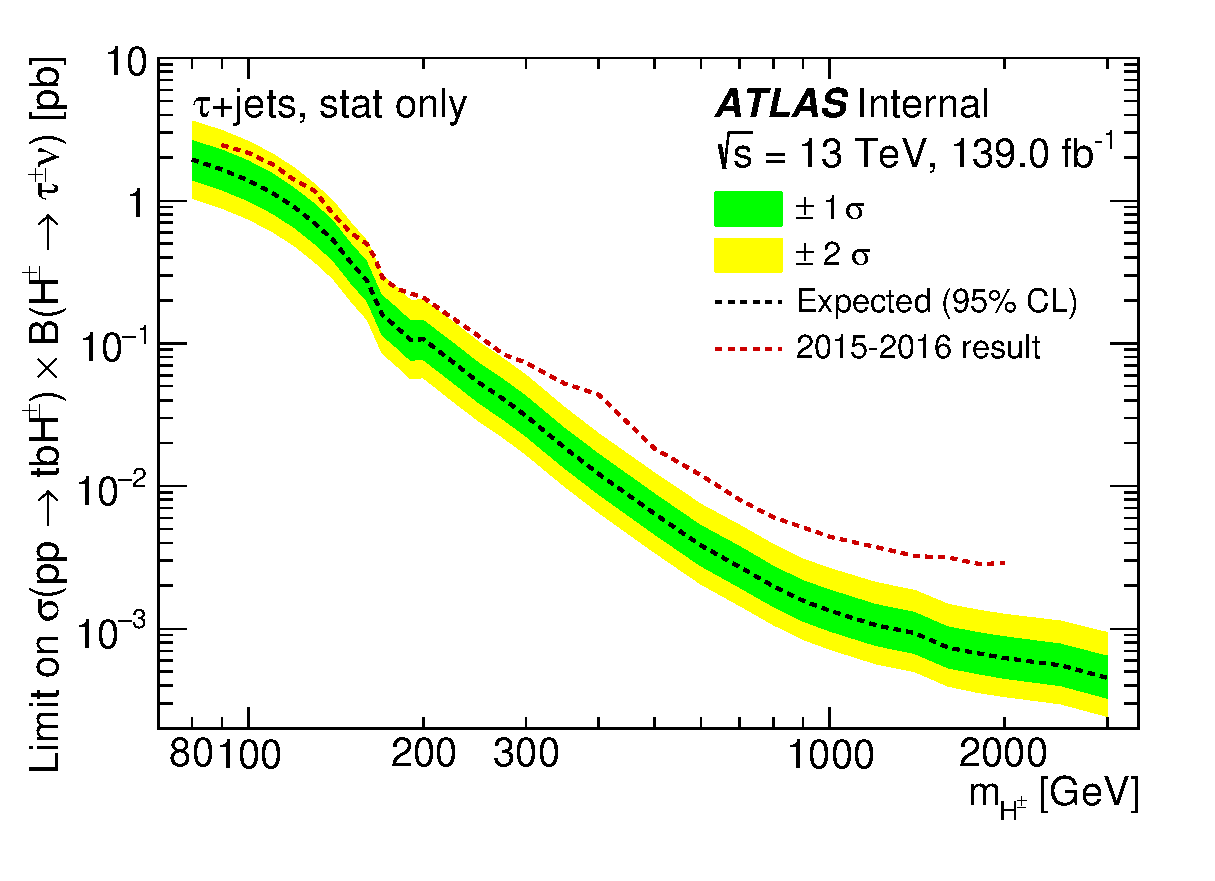
\includegraphics[width=.5\textwidth]{chapters/chapter6_HPlus/images/Limits/taujets_fullmass.eps}}
		\subfloat[\label{fig:expected-limits-b}]{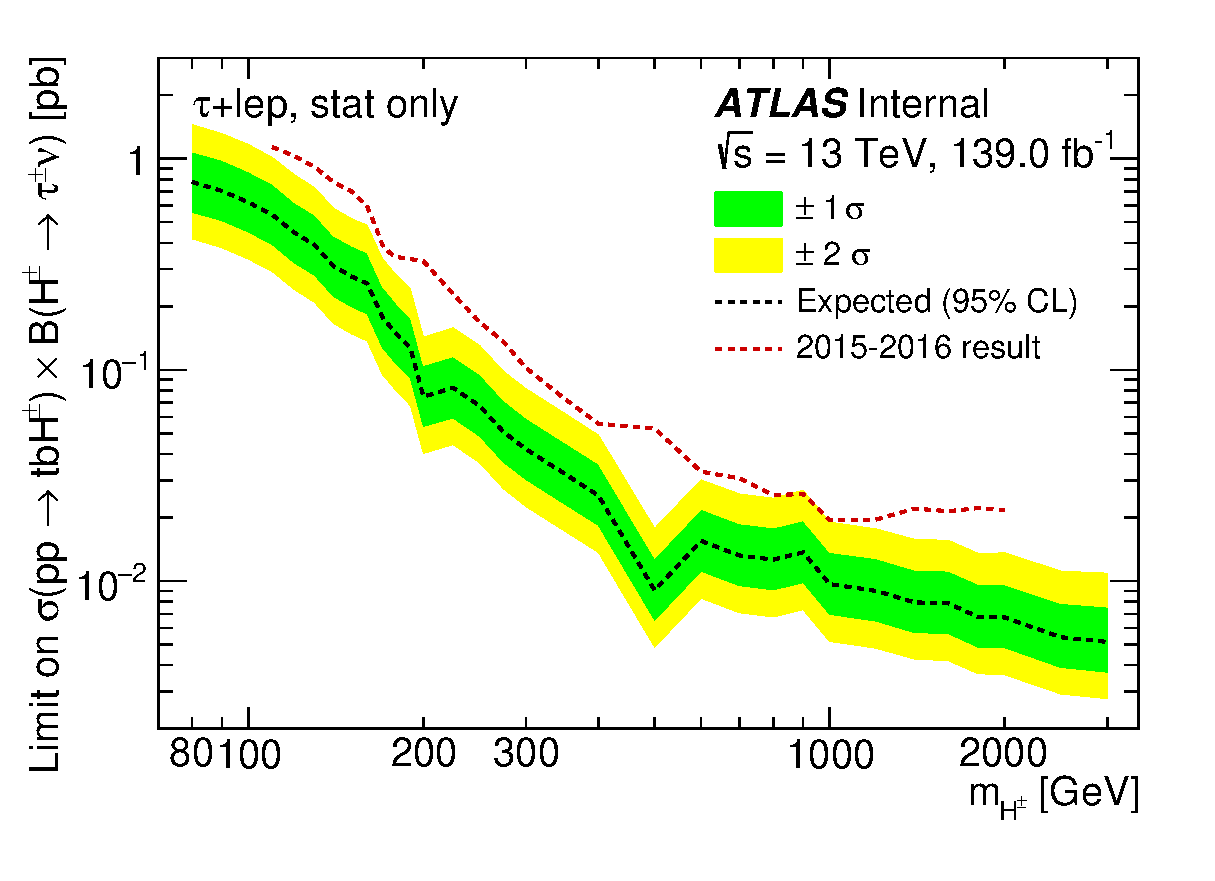
\includegraphics[width=.5\textwidth]{chapters/chapter6_HPlus/images/Limits/taulep_fullmass.eps}} \\
		\subfloat[\label{fig:expected-limits-c}]{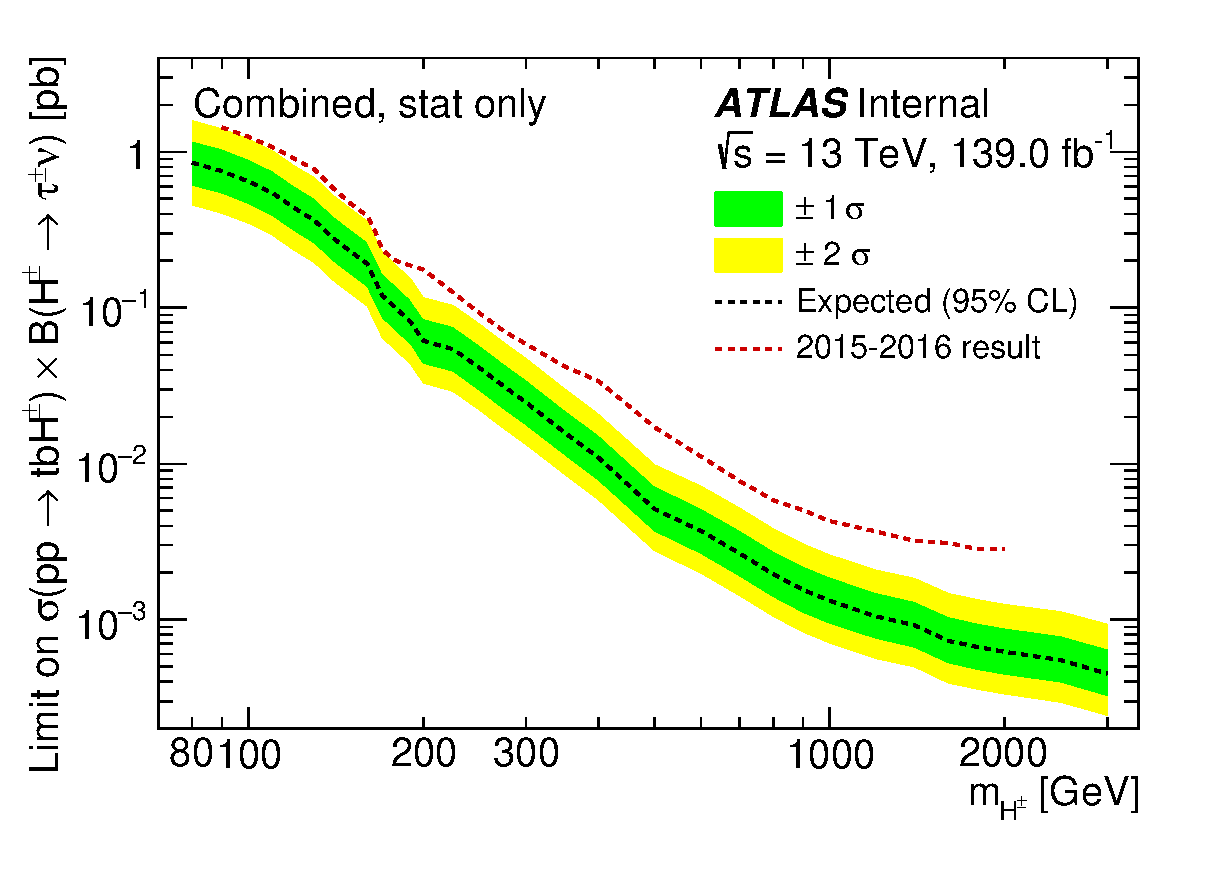
\includegraphics[width=\textwidth]{chapters/chapter6_HPlus/images/Limits/combined_fullmass.eps}}
		\caption{\label{fig:expected-limits} 
		Expected 95\% CL exclusion limits on $\sigma(\pp\to tb\Hpm)\times \mathrm{\cal{B}}(\Hpm \to \tau \nu)$ as a function of the charged Higgs boson mass in \LUMI of \pp collision data at \sqs in the \taujets signal region (a), \taulep signal region (b), and the combination of the \taujets and \taulep signal regions (c). In the case of the expected limits, one- and two-standard-deviation uncertainty bands are also shown. As a comparison, the expected exclusion limits obtained with the dataset collected in 2015 and 2016~\cite{hpm-previous} are also shown.
		 }
		\end{figure}